% !TEX root=./dummy-02.tex

\chapter{基于对电子方法的双杂化能量泛函实现与测评}
\label{sec.2.title}

\section{引言}

分子体系的基态能量始终是计算化学所关心的根本问题。只有准确地描述分子基态能量,才有可能准确描述分子自由能等热力学性质,并进而将计算结果应用于反应动力学、分子动力学、精细光谱等各种具体的化学或物理问题。目前主流的对分子体系基态性质描述的理论体系,有 post-HF、DFT、QMC 等。由于 DFT 的近似方法相比于其它理论框架下的方法而言,在相同的计算资源消耗下,可以对更大的分子体系作计算、并有更高的精度,即计算消耗与精度的性价比高;因此,密度泛函近似在计算化学应用受到广泛的欢迎与使用。在第一章绪论中,也回顾到密度泛函近似的其中一个分支,双杂化泛函,在涉及主族化学的各类反应能量、弱相互作用、几何结构、分子振动与谱学问题有良好的表现。

但密度泛函近似仍然存在一些困难。目前主流的密度泛函可以依据开发模式分为两类:经验参数拟合的、与纯理论模型的。一般来说,纯理论模型的泛函在测评数据集上的表现通常稍逊色\cite{Goerigk-Grimme.PCCP.2017};但对于经验参数拟合的泛函,可能在拟合范围外产生比较严重误差,即可泛化性通常较差\cite{Medvedev-Lyssenko.S.2017}。目前流行的大多数双杂化泛函,为保证一定的泛化能力,可以采用的策略是使用较少的参数数量,如 XYG$n$\cite{Zhang-Xu.JPCL.2021} 或 DSD 系列\cite{Kozuch-Martin.JCC.2013}等泛函;或者采用复杂的参数拟合策略,如 ωB97X-2\cite{Chai-Head-Gordon.JCP.2009} 或 ωB97M(2)\cite{Mardirossian-Head-Gordon.JCP.2018}等泛函。这些泛函的参数通常是针对主族化学体系的反应能与弱相互作用能数据集上拟合得到;但目前的测评中,这些泛函确实在原子密度\cite{Su-Xu.PNAS.2018}、偶极矩与极化率\cite{Hait-Head-Gordon.JCTC.2018, Hait-Head-Gordon.PCCP.2018}、化学位移\cite{Stoychev-Neese.JCTC.2018}等问题上有良好的结果,即表现出不错的泛化能力。但同时需要注意到,这些泛函仍然在以过渡金属为代表的一些计算问题上,数值表现通常还有提升的空间。

目前流行的双杂化泛函中,通常引入了 MP2 型相关能 $E_\mathrm{c}^\mathrm{MP2}$。若分子体系的 HOMO/LUMO gap 较小,则 $E_\mathrm{c}^\mathrm{MP2}$ 会产生严重的负误差。由于一部分过渡金属与多参考问题具有 HOMO/LUMO gap 较小的特性,因此双杂化泛函在这类问题上表现较差。波函数理论中,与 MP2 计算量相仿的电子对方法 IEPA\cite{Sinanoǧlu-Sinanoǧlu.ACP.1964, Nesbet-Nesbet.ACP.1965}、sIEPA\cite{Zhang-Scheffler.PRL.2016}、MP2/cr\cite{Dykstra-Davidson.IJQC.2000}\footnote{在 Dykstra and Davidson 原文\cite{Dykstra-Davidson.IJQC.2000}中提出了两种 MP2/cr 形式。原文的 MP2/cr-II 的计算需要自旋相同且同占据轨道角标的激发系数 $t_{i \bar i}^{a \bar b}$;这在 $\alpha, \beta$ 占据数不同的情形下难以合理地定义。在正文中,我们仅介绍与使用原文的 MP2/cr-I,并将其指代为 MP2/cr。} 等可以一定程度地避免 $E_\mathrm{c}^\mathrm{MP2}$ 型相关能的负误差。在双杂化泛函中引入这类相关能,有望在不加大计算量的同时,提高 HOMO/LUMO gap 较小体系问题的计算精度。这三类近似方法在本工作中统称为 EP 型相关能。

在理论层面,掺杂 MP2 型相关能的双杂化泛函基础,一般认为是 G\"orling-Levy 微扰理论的二阶近似。事实上,G\"orling-Levy 微扰理论建立起了密度泛函方法与波函数理论之间的联系,而这层联系不仅仅局限于二阶微扰、还可以与更高级的方法产生联系。从这个角度来看,在密度泛函中引入不同于 MP2 的其它波函数理论下的相关能,在 G\"orling-Levy 微扰理论的角度下是可以立足的。

基于这些认识,在本章工作中,将实现掺杂 IEPA 型相关能的双杂化泛函,并进行理论合理性说明与测评。\ref{sec.2.glpt2-theory}--\ref{sec.2.glpt2-dh} 小节将回顾 G\"orling-Levy 微扰理论,进一步详细地阐述其与波函数理论之间的关系,以及在密度泛函近似中引入波函数方法相关能的合理性。\ref{sec.3.ep} 节将回顾作为波函数理论的 IEPA 型相关能近似理论与计算实现。\ref{sec.2.iepa-results} 节将通过参数拟合的方式给出掺杂 IEPA 型相关能的双杂化泛函,并对部分主族化学、过渡金属体系、多参考问题进行测评,以及对参数优化过程进行讨论。

\section{理论背景}

\subsection{GLPT2 的理论框架}
\label{sec.2.glpt2-theory}

目前的双杂化泛函,大多数选用 GLPT2 作为其理论框架的支撑依据。我们也将使用 GLPT2 作为理论基础,并对此作简要的讨论。

密度泛函理论,相比于波函数理论,通常被认为可以以更低的计算代价实现较为准确的计算;但普适泛函 $F[\rho]$ 的获得途径并不清晰,因此如何系统性地逼近真实泛函,成为密度泛函发展的瓶颈之一。

对于易于求得、但需要借助于确切值的普适泛函 $F[\rho]$ 的 Kohn-Sham 波函数,与计算量巨大、但可以严格逼近确切值求得的真实波函数,绝热路径理论可以通过耦合常数 $\lambda$ 将两种波函数联系起来。该耦合常数 $\lambda$,以及其对应的 Hamiltonian 量定义如下:
\begin{equation}
  \label{eq.2.H-lambda-ac}
  \hat H_\lambda = \hat T + \lambda \hat V_\mathrm{ee} + \sum_i^{n_\mathrm{elec}} v_{\lambda}(\bm{r}_i)
\end{equation}
其中,$v_{\lambda}(\bm{r})$ 是随耦合常数 $\lambda$ 改变而不同的势函数;其作用是用于保持在不同的 $\lambda$ 下,$\hat H_\lambda$ 所给出的波函数的密度都等同于真实体系密度 $\rho(\bm{r})$。

如同波函数理论从 Hartree-Fock 波函数出发,经过微扰处理可以得到精确波函数;依耦合常数 $\lambda$ 展开的绝热路径上的微扰,也可以得到精确波函数;后者也称为 G\"orling-Levy 微扰框架\cite{Goerling-Levy.PRB.1993, Goerling-Levy.PRA.1994}。在该微扰框架下,定义 $\hat H_\lambda$ 对应的本征态为 $| \Psi_\lambda \rangle$;作为特例,真实波函数为 $| \Psi_{\lambda = 1} \rangle$,Kohn-Sham 波函数为 $| \Psi_{\lambda = 0} \rangle$;这两个波函数成功地通过耦合常数 $\lambda$ 得以联系。定义绝热路径上的被积函数
\begin{align}
  \mathcal{W}_{\lambda} [\rho] &= \langle \Psi_\lambda | \hat V_\mathrm{ee} | \Psi_\lambda \rangle \\
  \mathcal{W}_{\mathrm{c}, \lambda} [\rho] &= \mathcal{W}_{\lambda} [\rho] - E_\mathrm{x}^\mathrm{exact} [\rho] = \mathcal{W}_{\lambda} [\rho] - \langle \Psi_{\lambda = 0} | \hat V_\mathrm{ee} | \Psi_{\lambda = 0} \rangle
\end{align}
则普适泛函 $F[\rho]$ 中,唯一无法由 Kohn-Sham 波函数简单给出的相关能 $E_\mathrm{c} [\rho] = E_{\mathrm{c}, \lambda=1} [\rho]$,则由 Hellmann-Feynman 定理,可以展开为对耦合常数 $\lambda$ 的积分
\begin{equation}
  E_{\mathrm{c}, \lambda} [\rho] = \int_0^\lambda \mathcal{W}_{\mathrm{c}, \lambda} [\rho] \, \mathrm{d} \bm{r}
\end{equation}

假使 $E_{\mathrm{c}, \lambda} [\rho]$ 在以 $\lambda=0$ 为中心的邻域 $(0, 1]$ 下 Taylor 级数收敛,那么我们用下述记号表示该 Taylor 展开:
\begin{equation}
  \label{eq.2.e-c-lambda}
  E_{\mathrm{c}, \lambda} [\rho] = \sum_{n=2}^{\infty} \lambda^n E_\mathrm{GL}^{(n)} [\rho]
\end{equation}
作为具体的结果,G\"orling-Levy 微扰展开到第二阶时,其能量 $E_\mathrm{GL}^{(2)}$ 具有较为简单的形式:
\begin{align}
  \label{eq.2.GL2-W}
  E_\mathrm{GL}^{(2)} &= \frac{1}{2} \lim_{\lambda \rightarrow 0} \frac{\mathrm{d}^2}{\mathrm{d}^2 \lambda} E_{\mathrm{c}, \lambda} [\rho] = \frac{1}{2} \lim_{\lambda \rightarrow 0} \frac{\mathrm{d}}{\mathrm{d} \lambda} \mathcal{W}_{\mathrm{c}, \lambda} [\rho] \\
  \label{eq.2.GL2-def}
  &= \sum_{ia} \frac{\big| \langle i | \hat v_\mathrm{x}^\mathrm{NL} - v_\mathrm{x} | a \rangle \big|^2}{\varepsilon_i - \varepsilon_a} + \frac{1}{4} \sum_{ijab} \frac{\big| \langle ij || ab \rangle \big|^2}{\varepsilon_i + \varepsilon_j - \varepsilon_a - \varepsilon_b}
\end{align}
上式的 $v_\mathrm{x}^\mathrm{NL}$ 是非局域交换势算符。

对于式 (\ref{eq.2.GL2-W}),从更直观的角度来看,$\mathcal{W}_{\mathrm{c}, \lambda} [\rho]$ 作为关于 $\lambda$ 的函数,其在 $\lambda = 0$ 处的曲线斜率恰是 $2 E_\mathrm{GL}^{(2)}$;同时参考图 \ref{fig.2.adiabatic-curve}。而若进一步假设曲线 $\mathcal{W}_{\mathrm{c}, \lambda} [\rho]$ 关于 $\lambda$ 近似为直线,那么相关能就可以近似为 GLPT2 微扰能,即 $E_\mathrm{c} [\rho] \simeq E_\mathrm{GL}^{(2)}$。

\begin{figure}[h]
  \centering
  \includegraphics[width=0.5\textwidth]{assets/adiabatic-curve.jpg}
  \caption{绝热路径曲线示意图。下图取自文献\cite{Su-Xu.JCP.2014}。图中的 $W_{xc}^{\lambda}$ 即本文中的 $\mathcal{W}_{\lambda}$。图中的 $W'_{xc}{}^{0}$ 数值上等于本文中的 $2 E_\mathrm{GL}^{(2)}$。}
  \label{fig.2.adiabatic-curve}
\end{figure}

而对于式 (\ref{eq.2.GL2-def}),尽管 $E_\mathrm{GL}^{(2)}$ 的表达式相比于 MP2 相关能 $E_\mathrm{c}^\mathrm{MP2}$ 多出了关于 $v_\mathrm{x}^\mathrm{NL}$ 的单电子贡献项;但一般来说单电子贡献非常小\cite{DellaSala-Goerling.JCP.2001},同时 $v_\mathrm{x}$ 在实际计算中需要代价昂贵的响应函数方法\cite{Goerling-Goerling.PRL.1999}、或存在数值不稳定可能性的 KLI 方法\cite{Krieger-Iafrate.PRA.1992, DellaSala-Goerling.JCP.2001}或 OEP 方法\cite{Mori-Sanchez-Yang.JCP.2005};因此忽略上式的第一项,即单电子项,通常是可接受的。从而,$E_\mathrm{GL}^{(2)}$ 可以仅由第二项近似得到:
\begin{equation}
  E_\mathrm{GL}^{(2)} \simeq E_\mathrm{c}^\mathrm{MP2}
\end{equation}
这里 $E_\mathrm{c}^\mathrm{MP2}$ 是指基于 Kohn-Sham 波函数所给出的 MP2 相关能。

\subsection{GLPT2 与双杂化泛函}
\label{sec.2.glpt2-dh}

现在回到近似泛函的问题上。上一小节通过分析给出了 Kohn-Sham 相关能泛函与 MP2 相关能,在 $\mathcal{W}_{\mathrm{c}, \lambda} [\rho]$ 关于 $\lambda$ 接近线性、以及 $\hat v_\mathrm{x}^\mathrm{NL} - v_\mathrm{x}$ 算符效果接近于零的假设下,是非常相似的结论;即 $E_\mathrm{c} [\rho] \simeq E_\mathrm{GL}^{(2)} \simeq E_\mathrm{c}^\mathrm{MP2}$。当然现实情况下,$\mathcal{W}_{\mathrm{c}, \lambda} [\rho]$ 关于 $\lambda$ 并非严格线性,因此上述近似一般不能直接使用;但将 $E_\mathrm{c}^\mathrm{MP2}$ 作为杂化项掺入泛函,仍然是有所帮助的。这就构成了一般的 MP2 型双杂化泛函。但 MP2 相关能仅仅是最初步的其中一种引入 G\"orling-Levy 微扰方式;从具体实现上,如何引入 G\"orling-Levy 微扰、引入多大程度的近似能得到较精确地结果,都是值得讨论的话题。

理论上,我们可以获得依式 (\ref{eq.2.e-c-lambda}) 定义的 $\lambda=0$ 处各阶微扰能量;从而在 $\lambda$ 的级数收敛区间内给出最终的 $E_{\mathrm{c}, \lambda} [\rho]$。显然,若可以求得更高阶数的 G\"orling-Levy 微扰能 $E_\mathrm{GL}^{(n)}$ ($n > 2$),那么相关能的结果就更为精确。但如果对 G\"orling-Levy 微扰作更多分析,那么算符 $\hat H_\lambda$ 对耦合常数 $\lambda$ 的展开表达式为
\begin{equation}
  \hat H_\lambda = \left( \hat T - \sum_i^{n_\mathrm{elec}} v_\mathrm{s} (\bm{r}_i) \right) + \lambda \left( \hat V_\mathrm{ee} - \sum_i^{n_\mathrm{elec}} \big( v_\mathrm{J} (\bm{r}_i) + v_\mathrm{x} (\bm{r}_i) \big) \right) - \sum_{n=2}^\infty \lambda^n \sum_{i}^{n_\mathrm{elec}} v_\mathrm{c}^{(n)} (\bm{r}_i)
\end{equation}
其中,上式中出现的势函数是一些能量项对密度的函数变分:
\begin{equation*}
  v_\mathrm{s} (\bm{r}) = \frac{\delta T_\mathrm{s} [\rho]}{\delta \rho(\bm{r})} , \;
  v_\mathrm{J} (\bm{r}) = \frac{\delta J [\rho]}{\delta \rho(\bm{r})}, \;
  v_\mathrm{x} (\bm{r}) = \frac{\delta E_\mathrm{x}^\mathrm{exact} [\rho]}{\delta \rho(\bm{r})}, \;
  v_\mathrm{c}^{(n)} (\bm{r}) = \frac{\delta E_\mathrm{GL}^{(n)} [\rho]}{\delta \rho (\bm{r})}
\end{equation*}
由于在算符 $\hat H_\lambda$ 中存在算符 $\hat V_\mathrm{ee}$,因此,$n$ 阶的 G\"orling-Levy 计算量至少不会低于 M\o{}ller-Plesset 对应 $n$ 阶的微扰。

可以预见,G\"orling-Levy 微扰的计算代价是相当高的。但也需要指出,由于近年来近似算法 (特别是 RI 近似算法)、以及计算硬件 (特别是 DRAM 内存容量) 发展,MP2 相关能的计算在数十原子体系以内耗时不多于引入交换效应的 Kohn-Sham 自洽场计算;因此,对于 $n = 2$ 阶 G\"orling-Levy 微扰即 GLPT2,若近似为 MP2 相关则不会增加太多计算资源负担。而对于 $n = 3$ 阶的情形,现在确实有针对 MP3 相关能的计算所提出或适用的近似算法;这类算法通常基于 THC 或其它张量分解与缩并方法\cite{Hohenstein-Martinez.JCP.2012, Parrish-Sherrill.JCP.2012, Lee-Head-Gordon.JCTC.2020, Matthews-Matthews.JCTC.2020},但目前的效率仍然无法达到与自洽场计算齐平的程度\cite{Matthews-Matthews.JCP.2021}。考虑到杂化密度泛函近似近年来的巨大成功,得益于可以在较低自洽场级别的计算代价下获得相对精确的结果;其中计算代价小是非常重要的因素。因此,若 MP3 相关能的计算效率难以进一步提升,那么在可见的未来,基于 G\"orling-Levy 微扰理论所开发的实用的密度泛函,很可能不会引入\textbf{完整的} $n = 3$ 阶或更高阶微扰能量。

因此,若以 G\"orling-Levy 为基础发展泛函方法,仅引入 GLPT2 从计算资源消耗与精度平衡的角度上,是非常自然的想法。作为最基本的泛函模型,$\mathcal{W}_{\lambda}$ 若依 $\lambda$ 接近线性,则
\begin{equation}
  E_{\mathrm{xc}, \lambda} [\rho] = \lambda E_\mathrm{x}^\mathrm{exact}[\rho] + \lambda^2 E_\mathrm{GL}^{(2)} [\rho] + o(\lambda^3) \simeq E_\mathrm{x}^\mathrm{exact}[\rho] + E_\mathrm{GL}^{(2)} [\rho]
\end{equation}
当 $\lambda = 1$ 时,上述的 $E_{\mathrm{xc}, \lambda} [\rho]$ 就是真实体系的交换相关能 $E_{\mathrm{xc}} [\rho]$。但事实上,当相关能若仅引入 GLPT2 时,测评表现并不好\cite{Su-Xu.JCP.2014}。事实上,重新回顾式 (\ref{eq.2.GL2-W}) 的结论,微扰理论只能描述取到极限 $\lambda \rightarrow 0$ 时绝热路径曲线行为。若 $E_{\mathrm{c}, \lambda} [\lambda]$ 作为关于 $\lambda$ 的函数在 $(0, 1]$ 邻域上 Taylor 级数收敛,那么精确地描述 $\lambda \rightarrow 0$ 处越热路径曲线的行为 (可以精确计算 $\lambda \rightarrow 0$ 的各阶导数),也能给出正确的 $\lambda \in (0, 1]$ 下 $\mathcal{W}_{\lambda}$ 的结果;从而对 $\mathcal{W}_{\lambda}$ 作关于 $\lambda$ 的积分得到准确的 $E_\mathrm{xc}$。但在计算资源的限制下,如图 \ref{fig.2.adiabatic-curve} 所示,如果无法引入三阶或更高阶微扰能量,即只能相对精确地计算 $\mathcal{W}_{\lambda}$ 在 $\lambda = 0$ 处的函数值与斜率,我们只能得到非常粗糙的对 $\lambda = 0$ 附近 $\mathcal{W}_{\lambda}$ 的局部认识、而无法对整体形状有所把握;大多数分子的 $\mathcal{W}_{\lambda}$ 并不非常接近线性,那么若仅近似 $E_\mathrm{c} [\rho] \simeq E_\mathrm{GL}^{(2)} [\rho]$,自然无法给出好的测评表现。

为提升测评精度,也为了更好地对大多数类型分子的 $\mathcal{W}_{\lambda}$ 作合理建模以更好地逼近真实的 $E_\mathrm{xc} [\rho]$,其中一种有效且理论上相对严格的策略,是结合 G\"orling-Levy 微扰与传统的低阶密度泛函近似,对 $\mathcal{W}_{\lambda}$ 作合理的参数化。尽管传统的低阶泛函\footnote{低阶泛函 (low-rung functional) 指在“Jacob 阶梯”的第四阶或以下,即杂化泛函或以下的泛函。后文也经常使用该称法。}未必能正确地描述 $\mathcal{W}_{\lambda}$ 在 $\lambda \rightarrow 0$ 时的行为,但却因为对 $\mathcal{W}_{\lambda}$ 在 $\lambda \in [0, 1]$ 整体有良好的描述,传统泛函的 $E_\mathrm{xc} [\rho]$ 的结果通常相比于仅近似 $E_\mathrm{c} [\rho] \simeq E_\mathrm{GL}^{(2)} [\rho]$ 的 GLPT2 要更精确。如果在构造绝热路径曲线 $\mathcal{W}_{\lambda}$ 的过程中,在 $\lambda \rightarrow 0$ 时偏重 G\"orling-Levy 微扰理论、而在 $\lambda \rightarrow 1$ 时偏重传统泛函,那么可以取两者所长,获得比传统泛函近似或 GLPT2 更为精确的泛函。在这种新的泛函形式中,交换相关能同时有严格交换能 $E_\mathrm{x}^\mathrm{exact}$ 与二阶微扰相关能 $E_\mathrm{GL}^{(2)}$ 的掺杂:
\begin{equation}
  E_\mathrm{xc} = \int_0^\lambda \mathcal{W}_{\lambda} \, \mathrm{d} \lambda = E_\mathrm{xc}^\text{low-rung} + c_\mathrm{x} E_\mathrm{x}^\mathrm{exact} + c_\mathrm{c} E_\mathrm{GL}^{(2)}
\end{equation}
因此这类泛函近似成为双杂化泛函。

许多在测评结果上有优异表现的双杂化泛函,譬如 B2PLYP、XYG3 等,通过上述策略对将双杂化泛函近似合理化\cite{Grimme-Grimme.JCP.2006, Zhang-Goddard.PNAS.2009};但在实践中,则是直接对 $E_\mathrm{xc} [\rho]$ 中的参数 $c_\mathrm{x}, c_\mathrm{c}$ 在数据集下作拟合,而没有直接构造 $\mathcal{W}_{\lambda}$ 本身。以 PBE-ACDH\cite{Su-Xu.JCP.2014} 为代表的一类泛函,则是使用参数或模型构造 $\mathcal{W}_{\lambda}$ 并对 $\lambda$ 作积分,得到 $E_\mathrm{xc} [\rho]$。

需要指出,对绝热路径曲线 $\mathcal{W}_{\lambda}$ 作参数化或模型化后积分,从而在 $E_\mathrm{xc}$ 中引入 GLPT2 相关能,是双杂化泛函的其中一种理论基础。以 PBE0-DH\cite{Toulouse-Adamo.JCP.2011} 为代表的双杂化泛函,其理论基础并非构建于 $\lambda = 0$ 的 Kohn-Sham 轨道行列式下 G\"orling-Levy 微扰,而是构建于 $0 < \lambda < 1$ 下杂化泛函轨道行列式下的二阶微扰基础上\cite{Sharkas-Savin.JCP.2011};该理论引入绝热路径给出相关能的方式,与 G\"orling-Levy 微扰有些许不同。

不论是使用绝热路径、还是使用杂化泛函波函数下的微扰理论,都可以构造出双杂化泛函。但与低阶泛函中纯粹以理论模型驱动所构造 PBE、TPSS、SCAN 或他们对应的杂化泛函,在诸多数据集下测评表现相对于同等级参数拟合方法仍然有不少优势\cite{Goerigk-Grimme.PCCP.2017, Medvedev-Lyssenko.S.2017}的情况不同,存在经验参数的双杂化泛函近似通常要比纯理论模型驱动构造的泛函有更优异的测评表现\cite{Mehta-Goerigk.PCCP.2018}。因此,理论模型通常在双杂化泛函中扮演的角色,很可能是对双杂化泛函的合理化。若要提升双杂化泛函的测评数值表现,参数优化非常重要。

但理论模型仍然可以指导双杂化密度泛函的发展。目前在数值计算上的迹象表明,对于绝大多数体系,绝热路径曲线是凸曲线\cite{Frydel-Burke.JCP.2000, Fuchs-Burke.JCP.2005, Teale-Helgaker.JCP.2009,Teale-Helgaker.JCP.2010, Carrascal-Burke.JPCM.2015} (但该结论目前没有对任意体系成立的确切证明\cite{Crisostomo-Burke.LMP.2023}):
\begin{equation}
  \frac{\mathrm{d}^2}{\mathrm{d} \lambda^2} \mathcal{W}_{\lambda} \geqslant 0, \quad \lambda \in [0, 1] \quad \text{(conjecture)}
\end{equation}
这意味着图 \ref{fig.2.adiabatic-curve} 所示的绝热路径曲线 $\mathcal{W}_\lambda$,数值上必然不小于以 $E_\mathrm{x}^\mathrm{exact}$ 为零点、以 $2 E_\mathrm{GL}^{(2)}$ 为斜率的直线;进而对 $\mathcal{W}_\lambda$ 积分后,存在的关系式是
\begin{equation}
  E_\mathrm{xc} \geqslant E_\mathrm{x}^\mathrm{exact} + E_\mathrm{GL}^{(2)} \quad \text{(conjecture)}
\end{equation}
或者等价地,GLPT2 相关能相对于真实体系相关能必然有一定的负误差:
\begin{equation}
  E_\mathrm{GL}^{(2)} \leqslant E_{\mathrm{c}, \lambda=1} \quad \text{(conjecture)}
\end{equation}
作为具体的例子,在低阶密度泛函近似所给出的能量相对精确、且所给出的 Kohn-Sham 轨道足够精确的前提下,若要在能量计算中引入 GLPT2 相关能,那么对于下述泛函模型
\begin{equation*}
  E_\mathrm{xc}^\mathrm{DH} = c_\mathrm{x} E_\mathrm{x}^\mathrm{exact} + c_\mathrm{x}^\text{low-rung} E_\mathrm{x}^\text{low-rung} + c_\mathrm{c} E_\mathrm{GL}^{(2)} + c_\mathrm{c}^\text{low-rung} E_{\mathrm{c}, \lambda=1}^\text{low-rung}
\end{equation*}
我们应当预期
\begin{equation*}
  c_\mathrm{c} + c_\mathrm{c}^\text{low-rung} \leqslant 1 \quad \text{(conjecture)}
\end{equation*}
事实上,在 xDH@B3LYP 模型下的诸多泛函的优化结果印证了这个结论\cite{Zhang-Xu.JPCL.2021}。因此,要求 $c_\mathrm{c}, c_\mathrm{c}^\text{low-rung}$ 等相关能参数之和小于 1,是其中一种引入 GLPT2 相关能以构造双杂化泛函的限制条件。

同时,G\"orling-Levy 微扰理论本身是类似于波函数方法、通过微扰阶数增加而逐步逼近真实泛函的理论框架;因为微扰阶数的增加会导致计算资源的巨量消耗,现在的密度泛函近似避免使用更高阶的 G\"orling-Levy 微扰相关能而仅考虑 GLPT2。但注意到波函数理论中存在一些近似方法:它们在 M\o{}ller-Plesset 微扰或耦合簇理论的框架下,基于较低阶的近似,引入一部分计算量较小的高阶贡献。对应于 MP2 的计算消耗,介于 MP2 到 CCSD 的经典波函数方法有 IEPA\cite{Sinanoǧlu-Sinanoǧlu.ACP.1964, Nesbet-Nesbet.ACP.1965}、MP2/cr\cite{Dykstra-Davidson.IJQC.2000}、CC2\cite{Christiansen-Joergensen.CPL.1995} 等。在下一节中,我们将会回顾 IEPA 与 MP2/cr 方法,并表明这类方法的相关能将大于 MP2 的相关能。由于 GLPT2 相关能通常近似为基于 Kohn-Sham 轨道行列式的 MP2 相关能,而 GLPT2 相关能相对于真实体系的相关能 $E_\mathrm{c, \lambda=1}$ 总是负误差;同时,由于 G\"orling-Levy 微扰中包含 $\hat V_\mathrm{ee}$ 算符,因而一部分表达式预期与 M\o{}ller-Plesset 微扰有着同样的结构,在能量计算中引入高阶的基于 Kohn-Sham 轨道行列式的 M\o{}ller-Plesset 微扰能量是合理的;因此,在双杂化泛函近似中引入 IEPA 或 MP2/cr 等相关能,预期一定程度上可以化解 GLPT2 的负误差,并且是理论上合理的。

\subsection{电子对方法}
\label{sec.3.ep}

本工作考虑的 IEPA 方法与 MP2/cr 方法,从计算过程而言,都是基于占据电子成对效应而实现;因此我们统称这两类方法为电子对或 EP 方法。在将这类电子对方法引入密度泛函前,这里将在波函数理论下,介绍电子对方法的部分理论基础与性质。

若参考态为 Hartree-Fock 基态 $| 0 \rangle$,且依据 Brillouin 定理的推论认为在 Fock 算符下的一次激发态可以近似忽略,那么真实的、含有相关效应的波函数可以写为
\begin{equation}
  | \Psi \rangle = | 0 \rangle + \sum_{ijab} t_{ij}^{ab} | {}_{ij}^{ab} \rangle + \cdots
\end{equation}
上式中,$| {}_{ij}^{ab} \rangle$ 表示 Hartree-Fock 二次激发波函数 $a_a^\dagger a_b^\dagger a_j a_i | 0 \rangle$;$a_i, a_j$ 表示对占据轨道 $i, j$ 的湮灭算符、$a_a^\dagger, a_b^\dagger$ 表示对非占轨道的产生算符。在这里,$t_{ij}^{ab}$ 称为二次激发系数 (对于耦合簇理论,也称为二次簇算符系数)。对于本工作所提及的所有 post-HF 方法,在忽略一次激发态的前提下,相关能总是可以表示为二次激发系数与双电子积分的乘积和:
\begin{equation}
  E_\mathrm{c} = \frac{1}{4} \sum_{ijab} t_{ij}^{ab} \langle ij || ab \rangle
\end{equation}
因此,对二次激发系数 $t_{ij}^{ab}$ 计算方式的差异,区分了不同 post-HF 方法。

在本工作中,我们涉及的电子对方法是 IEPA 及其变种 sIEPA、以及 MP2/cr。大体来说,这些方法可以通过精确的方法一步一步近似得到。依照精度与计算消耗从大到小的排序,
\begin{itemize}[nosep]
  \item \textbf{Full-CI。}该方法将所有基于 Fock 算符下基态下的激发态作为变分空间,对分子体系的 Hamilton 算符 $\hat H$ 求取变分极小。在有限基组下,若不考虑溶剂化、分子振动、精细光谱以及其它实验化学影响下,该方法是最精确的计算化学方法;
  \item \textbf{CCD}\cite{Coester-Coester.NPB.1958, Coester-Kuemmel.NPB.1960, Cizek-Cizek.JCP.1966, Cizek-Paldus.IJQC.1971}\textbf{。}将高次 Hartree-Fock 激发态 (在 Fock 算符下的激发) 近似为二次簇算符的耦合。该方法满足正交不变性与大小延展性等重要的物理条件,且计算精度相对较高;但需要多次 $O(n_\mathrm{occ}^2 n_\mathrm{vir}^4)$ 复杂度的计算、且内存资源消耗巨大。
  \item \textbf{CEPA}\cite{Ahlrichs-Ahlrichs.CPC.1979}\textbf{。}将 CCD 簇算符系数方程中的部分项近似为零,以对计算过程中复杂度为 $O(n_\mathrm{occ}^2 n_\mathrm{vir}^4)$ 的巨量计算与内存消耗的项作非占轨道的解耦,从而仅耦合占据电子对。该方法以牺牲一定的精度与正交不变性为代价,换取计算效率的改善、并仍然保证大小延展性的性质。由于解耦非占轨道的方式不唯一,CEPA 存在四种不同的近似形式。
  \item \textbf{CPF}\cite{Ahlrichs-Ehrhardt.JCP.1985}\textbf{。}该方法是基于 CID 的改善。CPF 方法中,变分所涉及到的分母不同于波函数归一化量 $\langle \Psi | \Psi \rangle$,而是电子对的相关波函数的归一化量。该方法也具有大小延展性,且与 CEPA(1) 方法有所联系。
  \item \textbf{IEPA}\cite{Sinanoǧlu-Sinanoǧlu.ACP.1964, Nesbet-Nesbet.ACP.1965}\textbf{。}以 CEPA(2) 为基础,进一步地解耦成对占据轨道。
  \item \textbf{MP2/cr}\cite{Dykstra-Davidson.IJQC.2000}\textbf{。}以 CPF 为基础,忽略部分残差项近似而来。亦可以 CEPA(1) 为基础,通过激进的近似给出。
  \item \textbf{MP2}\cite{Moeller-Plesset.PR.1934}\textbf{。}对于所有上述涉及到的方法,在求取激发系数 $t_{ij}^{ab}$ 时忽略所有二阶及以上的微扰项、或在求取相关能时忽略所有三阶及以上的微扰项。
\end{itemize}

简要回顾 IEPA 与 MP2/cr 的具体表达式。对于 IEPA 方法,其能量可以拆解为成对占据电子的贡献总和:
\begin{equation}
  E_\mathrm{c}^\mathrm{IEPA} = \frac{1}{2} \sum_{ij} e_{ij}
\end{equation}
电子对 $ij$ 的相关能则表示为
\begin{equation}
  e_{ij} = \frac{1}{2} \sum_{ab} \frac{|\langle ij || ab \rangle|^2}{D_{ij}^{ab} + e_{ij}} \quad \text{(IEPA)}
\end{equation}
其中,$D_{ij}^{ab}$ 是轨道能差 $\varepsilon_i + \varepsilon_j - \varepsilon_a - \varepsilon_b$。作为参照,MP2 的电子对相关能表示为
\begin{equation}
  e_{ij} = \frac{1}{2} \sum_{ab} \frac{|\langle ij || ab \rangle|^2}{D_{ij}^{ab}} \quad \text{(MP2)}
\end{equation}
从程序实现的角度,IEPA 方法需要迭代、而 MP2 方法则可以一次性地给出电子对能量。对于 HOMO/LUMO gap 较小的体系,若此时的 $i, j$ 代表 HOMO 轨道、$a, b$ 代表 LUMO 轨道,则 $D_{ij}^{ab}$ 的数值较小、但 $e_{ij}$ 会因为作为分母的 $D_{ij}^{ab}$ 较小而有较大的数值。对于 MP2 方法,当 $D_{ij}^{ab}$ 接近零时,$e_{ij}$ 将会接近负无穷大;但对于 IEPA 方法,由于较大数值的 $e_{ij}$ 也在分母中,因而避免了 $e_{ij}$ 趋于负无穷大的趋势。因此,IEPA 方法在 HOMO/LUMO gap 较小的体系,特别是分子解离曲线问题上,相对于 MP2 有更好的表现\cite{Zhang-Scheffler.NJP.2016, Zhang-Scheffler.PRL.2016}。

对于 MP2/cr 方法,它相对于 MP2 方法而言,电子对相关能缩放了一个比例 $N_{ij}$:
\begin{equation}
  \label{eq.2.eij-MP2cr}
  e_{ij} = \frac{1}{2} \sum_{ab} \frac{1}{N_{ij}} \frac{|\langle ij || ab \rangle|^2}{D_{ij}^{ab}} \quad \text{(MP2/cr)}
\end{equation}
其中,比例系数定义为
\begin{equation}
  \label{eq.2.Nij-MP2cr}
  N_{ij} = 1 + \frac{1}{2} \sum_{kab} \big( (t_{ik}^{ab})^2 + (t_{jk}^{ab})^2 \big) \quad \text{(MP2/cr)}
\end{equation}
从程序实现的角度,MP2/cr 与 MP2 方法一样,可以一次性地给出电子对能量。对于 HOMO/LUMO gap 较小的体系,由于置于分母中的比例系数 $N_{ij}$ 中包含较大的激发张量平方 $(t_{ij}^{ab})^2$,因此也可以避免 $e_{ij}$ 过快地区域负无穷大的趋势。该方法同样在分子解离曲线上,相比于 MP2 有更好的表现\cite{Dykstra-Davidson.IJQC.2000}。

由于 IEPA 与 MP2/cr 方法均是增加分母的绝对值;而相关能本身是负值,因此这两个方法一定会给出比 MP2 相关能更大的 (绝对值上更小的) 相关能。回顾到先前关于绝热路径的讨论,可以认为这类方法相对于 MP2 考虑了更多的高阶微扰贡献、且有希望更好地满足绝热路径曲线的凸性。我们预期在密度泛函中引入这类电子对方法的相关能形式,特别在 HOMO/LUMO gap 较小的体系,有望提升泛函的测评精度。

\section{实现细节}

\subsection{数据集与误差量标}

在本工作中,我们将使用 GMTKN55 全数据集\cite{Goerigk-Grimme.PCCP.2017}与 Minnesota 2015 其中五个数据子集\cite{Yu-Truhlar.PCCP.2015} (MR-MGM-BE4、MR-MGN-BE17、MR-TM-BE13、SR-MGM-BE9、SR-TM-BE17),作为泛函表现的量标。这两个数据集的子集说明列于表 \ref{tab.2.subset-detail}。其中,Minnesota 2015 数据子集中的“单参考”与“多参考”,是指在波函数或密度泛函方法计算下,依据一定的指标特征\cite{Lee-Taylor.IJQC.1989, Schultz-Truhlar.JPCA.2005, Zhao-Truhlar.JCTC.2006, Tishchenko-Truhlar.JCTC.2008},若体系的 Hartree-Fock 参考态在考虑相关效应的波函数中占据较大的比例,则称该体系为单参考 (single-reference) 的;否则是多参考 (multi-reference) 的。

\begin{table}[h]
\centering
\caption{测评数据集概况与参数拟合权重。}
\label{tab.2.subset-detail}
\widetabular{
  \begin{tabular}{llllr}
  \toprule
  数据集         & 子集名称\tnote{a}        & 化学问题        & 反应数据数 & 权重 \\
  \midrule
  GMTKN55        & Sub1        & 基本性质与小体系反应能 & 473 & 48\%\tnote{b} \\
                & Sub2        & 大体系反应能与异构能  & 243 &  \\
                & Sub3        & 反应势垒        & 194 &  \\
                & Sub4        & 分子间非共价相互作用  & 291 &  \\
                & Sub5        & 分子内非共价相互作用  & 304 &  \\ \midrule
  Minnesota 2015 & MR-MGM-BE4  & 多参考主族金属键能   & 4 & 12\% \\
                & MR-MGN-BE17 & 多参考主族非金属键能  & 17 & 8\% \\
                & MR-TM-BE13  & 多参考过渡金属键能   & 13 & 12\%  \\
                & SR-MGM-BE9  & 单参考主族金属键能   & 9  & 8\%  \\
                & SR-TM-BE17  & 单参考过渡金属键能   & 17 & 12\%  \\
  \bottomrule
  \end{tabular}
}{
  \item[a] 对于 GMTKN55 数据集,这里列出的 Sub$n$ ($n = 1, 2, 3, 4, 5$) 是大子集;它囊括其它种类的小子集。在本工作中,我们将很少细致地考察 GMTKN55 的小子集测评情况;因此本工作一般称 GMTKN55 的大子集为子集。
  \item[b] GMTKN55 数据集所有子集的 WTMAD-2 权重。
}
\end{table}

测评 GMTKN55 所使用的误差量标是 WTMAD-2:
\begin{equation}
  \text{WTMAD-2} = \frac{1}{\sum_{i}^{n_\mathrm{sub}} N_i} \cdot \sum_{i}^{n_\mathrm{sub}} N_i \cdot \frac{\SI{56.84}{kcal.mol^{-1}}}{\overline{|\Delta E|}_i} \text{MAD}_i
\end{equation}
其中,上式的 $n_\mathrm{sub}$ 是测评数据集的小子集数量、$N_i$ 是小子集 $i$ 的反应数据数量、$\overline{|\Delta E|}_i$ 是小子集 $i$ 反应能参考值的平均绝对值、$\text{MAD}_i$ 是泛函近似在小子集 $i$ 上误差的平均绝对值。该测评量标使得反应前后能量差较大的情形 (譬如燃烧焓、键能、电离能等问题) 允许较大的能量误差、而能量差较小的情形 (譬如弱相互作用、配位效应、分子异构等问题) 则有更苛刻的精度要求,从而较好地平衡了不同反应类型的误差标准。

测评 Minnesota 2015 数据子集的误差量标是 MUEPB,即计算误差时先除以断键数量再取平均绝对值。因此,MUEPB 并非反应能量的误差量标、而是均摊到每个分子键后的键能误差量标。该量标不区分化学键种类,即对单键、双键、三键、配位键一视同仁。

需要指出的是,GMTKN55 数据集与 Minnesota 2015 数据集存在一定的重合。举例来说,Minnesota 2015 数据集中的 MR-MGN-BE17 (多参考主族非金属键能,测评 \ce{CO}、\ce{O2}、\ce{N2} 等主族小分子键解离能) 子集中部分分子收录到 GMTKN55 子集 Sub1 中的 W4-11 (Weizmann-4 原子化能) 小子集;MR-MGM-BE4 (多参考主族金属键能,测评 \ce{CaO}、\ce{MgS} 等体系的键解离能) 与 SR-MGM-BE9 (单参考主族金属键能,测评 \ce{AlCl3}、\ce{AlF3}、\ce{NaO} 等分子的键解离能) 子集的部分分子同时收录到 GMTKN55 子集 Sub1 中的 W4-11 与 ALKBDE10 (碱金属键解离能) 小子集。由于大多数经过经验参数拟合的泛函,其拟合数据集通常与 GMTKN55 较为接近,因此这类泛函在部分数据集 (特别是 MR-MGN-BE17 与 SR-MGM-BE9) 上的表现通常较好。而相应地,尽管 SR-TM-BE13 的计算体系被认为是单参考的,但绝大多数经验参数拟合的密度泛函近似没有将过渡金属纳入拟合数据中、或没有针对过渡金属问题对泛函表达式进行优化,因此多数泛函的测评结果较差。因此,从这部分的测评结果来看,计算体系是否纳入了近似泛函所使用的拟合数据集、以及这类计算问题是否以更大权重地被近似泛函所拟合,相比于计算问题与近似泛函是否同样有单参考的结构,对近似泛函的计算表现影响更重要。部分当前主流的双杂化泛函在 GMTKN55 数据集与 Minnesota 2015 数据集的测评结果列于表 \ref{tab.2.bench-current-gmtkn55-minnesota}。

\begin{sidewaystable}
\centering
\caption{现有泛函在 GMTKN55 全数据集与 Minnesota 2015 部分子集的测评结果。单位 \si{kcal.mol^{-1}}。}
\label{tab.2.bench-current-gmtkn55-minnesota}
\widetabular{
  \begin{tabular}{ld{1.3}d{1.3}d{2.2}d{2.2}d{2.2}d{2.2}d{2.2}d{2.2}}
  \toprule
  & \multicolumn{2}{c}{GMTKN55} & \multicolumn{5}{c}{Minnesota 2015\tnote{a}} & \\
  \cmidrule(lr){2-3} \cmidrule(lr){4-8}
  计算方法      &
  \multicolumn{1}{c}{disp.\tnote{b}} & \multicolumn{1}{c}{no disp.} &
  \multicolumn{1}{c}{MR-MGM-BE4} & \multicolumn{1}{c}{MR-MGN-BE17} & \multicolumn{1}{c}{MR-TM-BE13} & \multicolumn{1}{c}{SR-MGM-BE9} & \multicolumn{1}{c}{SR-TM-BE17} &
  \multicolumn{1}{c}{Weighted Error\tnote{c}} \\
  \midrule
  B2GPPLYP        
  & 3.72\tnote{d} & 6.26\tnote{d} & 5.11       & 2.94        & 5.87       & 1.82       & 9.50       & 4.62     \\
  B2PLYP          
  & 5.10\tnote{d} & 8.70\tnote{d} & 6.77       & 2.35        & 4.69       & 2.29       & 9.29       & 5.31     \\
  DSD-BLYP-D3(BJ)   
  & 3.50\tnote{d} & 5.96\tnote{d} & 6.44       & 2.39        & 8.29       & 1.99       & 11.76      & 5.21     \\
  DSD-PBEP86-D3(BJ) 
  & 2.45\tnote{d} & 4.21\tnote{d} & 5.83       & 2.09        & 7.47       & 2.12       & 11.97      & 4.55     \\
  PBE-QIDH        
  & 4.47\tnote{e} & 5.61\tnote{e} & 3.24       & 5.65        & 7.39       & 3.44       & 12.92      & 5.70     \\
  PBE0-DH         
  & 5.54\tnote{e} & 8.13\tnote{e} & 6.54       & 7.58        & 5.59       & 4.07       & 10.02      & 6.25     \\
  TPSS-QIDH       
  & 4.47\tnote{e} & 6.50\tnote{e} & 3.64       & 9.90        & 7.27       & 3.66       & 12.21      & 6.00     \\
  TPSS0-DH        
  & 5.86\tnote{e} & 9.77\tnote{e} & 8.05       & 14.08       & 6.46       & 4.69       & 9.92       & 7.25     \\
  ωB97X-2(TQZ)
  & 3.06\tnote{f} & 2.80\tnote{f} & 4.65       & 2.99        & 6.77       & 1.47       & 10.15      & 4.41     \\
  RS-PBE-P86      
  & -               & -               & 2.77       & 4.20        & 7.44       & 3.30       & 15.91      & -        \\
  XYG3            
  & -               & 3.39\tnote{a} & 16.93      & 1.81        & 10.67      & 1.59       & 5.56       & 5.88     \\
  XYG6            
  & -               & 2.18\tnote{a} & 22.85      & 3.97        & 13.20      & 1.78       & 7.23       & 6.70     \\
  XYG7            
  & -               & 2.01\tnote{a} & 17.81      & 2.63        & 12.12      & 2.55       & 6.75       & 5.78     \\
  xDH-PBE0        
  & -               & -               & 18.02      & 4.54        & 8.82       & 2.16       & 10.29      & -        \\
  \bottomrule
  \end{tabular}
}{
  \item[a] Minnesota 2015 部分子集、以及 GMTKN55 下 xDH@B3LYP 模型下泛函 (包括 XYG3、XYG6、XYG7) 的测评数据取自本工作。除 DSD-BLYP-D3(BJ) 与 DSD-PBEP86-D3(BJ) 外,其余泛函在 Minnesota 2015 集合下的测评没有使用色散矫正。XYG3、XYG6、XYG7 的测评结果与文献\cite{Zhang-Xu.JPCL.2021}有一定差距,这是因为本工作与该文献使用了不同的基组与冻核近似规则。
  \item[b] 色散矫正模型均选用 DFT-D3(BJ)。
  \item[c] 在计算加权误差时,选取 GMTKN55 误差较低的数值 (一般来说,若有色散矫正,则使用矫正后的 WTMAD-2 误差),测评结果。
  \item[d] 数据取自文献\cite{Goerigk-Grimme.PCCP.2017}。
  \item[e] 数据取自文献\cite{Mehta-Goerigk.PCCP.2018}。
  \item[f] 数据取自文献\cite{Santra-Martin.JPCA.2019}。
}
\end{sidewaystable}

在后续的工作中,我们将对上述数据集进行参数拟合,构造新的密度泛函。该拟合过程选用的误差量标是 GMTKN55 数据集的 WTMAD-2 误差、与 Minnesota 2015 五个子数据集的 MUEPB 误差的加权 (Weighted Error)。权重列于表 \ref{tab.2.basis-gmtkn55}。该权重是人为设置的;其设置方式反映的是我们对新泛函所能应用的化学问题范围与能力的期许。
\begin{itemize}[nosep]
  \item 设置 GMTKN55 数据集的权重为 48\%,目的是期望参数拟合后的泛函仍然能在诸多主族化学问题中有良好的表现;
  \item 设置 MR-MGM-BE4、MR-TM-BE13、SR-TM-BE17 数据集的权重为 12\%,目的是期望在不严重破坏诸多主族化学计算问题的表现的同时,针对现有泛函难以计算准确的问题作改善;对于表 \ref{tab.2.bench-current-gmtkn55-minnesota} 中所测评的 xDH@B3LYP 模型泛函,除了单参考、多参考过渡金属键解离问题外,主族碱金属的表现也欠佳,因此对这三类化学体系都加以较大的拟合权重;
  \item 设置 MR-MGN-BE17、SR-MGM-BE9 数据集的权重为 8\%;这两类计算问题下 xDH@B3LYP 模型泛函的测评表现良好;权重数值设置得较小,目的是避免对过渡金属键解离问题过拟合。
\end{itemize}

\subsection{数据集计算细节}

双杂化能量泛函的计算使用 \textsc{dh} 程序 v0.1.9 与 commit 80ca9e8;该程序的基础框架是 \textsc{PySCF} (ver 2.2.1)。在正文中出现的计算任务没有使用波函数稳定性分析,所有自旋投影 $S_z$ 为零的体系使用限制性 Kohn-Sham 轨道、而 $S_z$ 非零的体系使用非限制性 Kohn-Sham 轨道进行计算。

GMTKN55 数据集计算选用的基组列于表 \ref{tab.2.basis-gmtkn55}。GMTKN55 计算所选用的冻核近似规则列于表 \ref{tab.2.fc-gmtkn55}。Minnesota 2015 数据集所选用的基组是 def2-QZVPP,冻核近似规则为表 \ref{tab.2.fc-gmtkn55} 中的 FC-2 规则。

本工作选用 \textsc{SciPy}\cite{Virtanen-Vazquez-Baeza.NM.2020} 进行泛函参数的优化。优化算法选用 L-BFGS-B 算法\cite{Byrd-Zhu.SJSC.1995},收敛判标是参数梯度模长 (\verb|gtol|) 小于 $10^{-5}$。本工作没有进行严格的全局优化;对于后文表 \ref{tab.2.coeff-xyg6-1-weighted-error} 的参数,优化过程是非对电子能矫正项以 XYG6 的参数、对电子能占比微扰能比例以 0.7 作为初始参数;对于 \ref{sec.2.proportion-iepa-like}、\ref{sec.2.proportion-exchange}、\ref{sec.2.propotion-dataset} 等小节中的参数优化问题与图像绘制过程,则以其对应的原始泛函参数、或图中相邻的数据点作为初始参数优化。

\begin{table}[h]
\centering
\caption{GMTKN55 数据集计算所使用的基组}
\label{tab.2.basis-gmtkn55}
\widetabular{
  \begin{tabular}{lll}
    \toprule
    基组类型 & 基组 & 对应的子集 \\
    \midrule
    Conventional        & def2-QZVPPD               & WATER27, RG18, IL16, G21EA, \\
                        &                           & BH76, BH76RC, AHB21, ISOL24  \\
                        & def2-TZVPP                & C60ISO, UPU23 \\
                        & def2-QZVPP                & other 45 subsets of GMTKN55 \\
    \midrule
    Auxiliary  & daug-def2-universal-jkfit & WATER27, RG18, IL16, G21EA, \\
    (RI-JK)    &                           & BH76, BH76RC, AHB21, ISOL24 \\
                        & def2-universal-jkfit      & other 47 subsets of GMTKN55 \\
    \midrule
    Auxiliary & def2-QZVPPD-rifit         & WATER27, RG18, IL16, G21EA, \\
    (RI-MP2)  &                           & BH76, BH76RC, AHB21, ISOL24 \\
                        & def2-TZVPP-rifit          & C60ISO, UPU23 \\
                        & def2-QZVPP-rifit          & other 45 subsets of GMTKN55 \\
    \bottomrule
  \end{tabular}
}{}
\end{table}

\begin{table}[h]
\centering
\caption{GMTKN55 数据集计算所使用的冻核近似规则 (Rn 前元素)}
\label{tab.2.fc-gmtkn55}
\widetabular{
  \begin{tabular}{cccccc}
    \toprule
    \multicolumn{2}{c}{FC-0\tnote{a}}  &
    \multicolumn{2}{c}{FC-1\tnote{b}}  &
    \multicolumn{2}{c }{FC-2\tnote{c}}  \\
    \cmidrule(lr){1-2} \cmidrule(lr){3-4} \cmidrule(lr){5-6}
    冻结电子 & 元素 & 冻结电子 & 元素 & 冻结电子 & 元素 \\
    \midrule
    0              & H--Be    & 0              & H--Be    & 0              & H--B     \\
    2              & B--Mg    & 2              & B--Ar    & 2              & C--Si    \\
    10             & Al--Zn   & 10             & K--Kr    & 10             & P--As    \\
    18             & Ga--Sr   & 18             & Rb--Cd   & 18             & Se--Cd   \\
    28             & Zr--Cd   & 28             & In--Xe   & 28             & Cd--Te   \\
    36             & In--Yb   & 36             & Cs--Yb   & 36             & I--Yb    \\
    46             & Lu--Hg   & 46             & Lu--Hg   & 46             & Lu--Hg   \\
    68             & Tl--Rn   & 60             & Tl--Rn   & 60             & Tl--Rn   \\
    \bottomrule
  \end{tabular}
}{
  \item[a] 该规则取自 ORCA (ver 5.0.2) 默认冻核近似规则\cite{Neese-Neese.WCMS.2012, Neese-Neese.WCMS.2018, Neese-Neese.WCMS.2022},并应用于除下述特例外的所有其它子集。
  \item[b] 该规则应用于 HEAVY28 子集。
  \item[c] 该规则取自文献\cite{Santra-Martin.JPCA.2019}。对金属与过渡金属 (B, Si, Ge, As, Sb, Te),该规则将最靠近价层的电子纳入 post-SCF 的相关能计算;而对于其它非金属,仅有价层电子纳入 post-SCF 的相关能计算。该规则应用于 ALK8、ALKBDE10、HAL59、HEAVYSB11、MB16-43 子集。
}
\end{table}

\subsection{解离曲线计算细节}

分子解离曲线问题的计算中,除作为参考值的 DMC 方法外,其它方法选择 cc-pV5Z 基组。MP2、CCSD、CCSD(T) 方法使用传统四中心二电子积分计算,其它方法使用 RI-JK 与 RI-MP2 算法并使用辅助基组 cc-pV5Z-jkfit 与 cc-pV5Z-rifit。计算程序是 \textsc{PySCF} 与 \textsc{dh} commit 80ca9e8。

对于 DMC 方法,首先选用 ccecp-cc-pVQZ 基组在 \textsc{PySCF} 下给出 CASSCF 的波函数初猜;随后在 \textsc{PyQMC} 程序下先进行 1000 组态数量的 15 次 VMC 过程;其次进行 10000 组态数量的 4000 次 DMC,并舍弃前 200 次运行结果作能量计算;最后将时间步长为 0.02、0.01、0.005、0.0025、0.001 Hartree 的 DMC 结果线性外推到 0 时间步长的情形。

本工作的分子解离曲线势能面取用相对能量,且在正文中,所有计算限制使用闭壳层波函数。

\section{结果与讨论}
\label{sec.2.iepa-results}

\subsection{XYG6+1 模型双杂化近似泛函的参数优化}

本工作将基于 xDH@B3LYP 模型\cite{Zhang-Xu.JPCL.2021},作新泛函的拟合。回顾到 xDH@B3LYP 模型定义为
\begin{align}
  E_\mathrm{xc}^\text{xDH@B3LYP} &= a_1 E_\mathrm{x}^\mathrm{exact} + a_2 E_\mathrm{x}^\mathrm{S} + a_3 E_\mathrm{x}^\mathrm{B88} + a_4 E_\mathrm{c}^\mathrm{VWN3} + a_5 E_\mathrm{c}^\mathrm{LYP} \notag \\
  &\quad + a_6 E_\mathrm{c}^\text{OS-MP2} + a_7 E_\mathrm{c}^\text{SS-MP2}
\end{align}
其中,$E_\mathrm{x}^\mathrm{exact}$ 表示 (Generalized) Kohn-Sham 轨道下的严格交换能,$E_\mathrm{x}^\mathrm{S}$ 表示 LDA 型 Slater 交换能\cite{Bloch-Bloch.ZP.1929,Dirac-Dirac.MPCPS.1930},$E_\mathrm{x}^\mathrm{B88}$ 表示 GGA 型 Becke88 交换能\cite{Becke-Becke.PRA.1988},$E_\mathrm{c}^\mathrm{VWN3}$ 表示 LDA 型 Vosko-Wilk-Nusair 相关能\cite{Vosko-Nusair.CJP.1980} (B3LYP 泛函的构成部分之一\cite{Becke-Becke.JCP.1993,Stephens-Frisch.JPC.1994}),$E_\mathrm{c}^\mathrm{LYP}$ 表示 Lee-Yang-Parr 相关能\cite{Lee-Parr.PRB.1988},$E_\mathrm{c}^\text{OS-MP2}$ 与 $E_\mathrm{c}^\text{SS-MP2}$ 分别代表基于参考态的自旋相反与自旋相同的 MP2 相关能。

xDH@B3LYP 模型总共有 7 个可变参数。XYG7 近似泛函的参数是通过对 GMTKN55 数据集的 WTMAD-2 量标进行优化所得到。而 XYG6 近似泛函的参数则是在下述限制条件下,对 WTMAD-2 量标优化得到:
\begin{equation}
  \label{eq.2.constrain-xyg6}
  a_1 + a_2 + a_3 = 1 \quad \text{(constrain on XYG6)}
\end{equation}

为引入 IEPA-like 相关能,我们引入额外的参数 $a_8$,用以控制 IEPA-like 相关能占总高阶微扰相关能的比例;该模型记为 xDH@B3LYP+1,其形式为
\begin{align}
  E_\mathrm{xc}^\text{xDH@B3LYP+1/cr} &= a_1 E_\mathrm{x}^\mathrm{exact} + a_2 E_\mathrm{x}^\mathrm{S} + a_3 E_\mathrm{x}^\mathrm{B88} + a_4 E_\mathrm{c}^\mathrm{VWN3} + a_5 E_\mathrm{c}^\mathrm{LYP} \notag \\
  &\quad + (1 - a_8) (a_6 E_\mathrm{c}^\text{OS-MP2} + a_7 E_\mathrm{c}^\text{SS-MP2}) \notag\\
  &\quad + a_8 (a_6 E_\mathrm{c}^\text{OS-IEPA-like} + a_7 E_\mathrm{c}^\text{SS-IEPA-like})
\end{align}
上式的 $E_\mathrm{c}^\text{SS-IEPA-like}$ 与 $E_\mathrm{c}^\text{OS-IEPA-like}$ 分别代表基于参考态的自旋相反与自旋相同的 IEPA-like 型的相关能。根据引入到泛函近似的 IEPA-like 种类的不同,它可以代表 MP2/cr ($E_\mathrm{c}^\mathrm{MP2/cr}$)、sIEPA ($E_\mathrm{c}^\mathrm{sIEPA}$) 与 IEPA ($E_\mathrm{c}^\mathrm{IEPA}$) 相关能。MP2 与 IEPA-like 在均是微扰形式的相关能;我们也会用记号 PT 表示总微扰相关效应。

在本工作中,我们将始终对 xDH@B3LYP+1 模型引入 XYG6 的限制 (\ref{eq.2.constrain-xyg6}),并称其为 XYG6+1 模型。对 GMTKN55 全集与 Minnesota 2015 的五个子集进行加权拟合后,XYG6+1/cr、XYG6+1/sIEPA 与 XYG6+1/IEPA 模型的泛函参数如表 (\ref{tab.2.coeff-xyg6-1-weighted-error}) 所示。

对于泛函系数,我们注意到 $E_\mathrm{x}^\mathrm{B88}$ 的比例通常小于零;这一现象也出现在 XYG7 对 GMTKN55 数据集的 WTMAD-2 误差量标参数拟合中。除此之外,代表 $E_\mathrm{c}^\text{IEPA-like}$ 占比的参数 $a_8$ 在 XYG6+1/sIEPA 与 XYG6+1/IEPA 中大于一,意味着在这些泛函中 $E_\mathrm{c}^\text{MP2}$ 的占比小于零;而在 XYG6+1/cr 中参数 $a_8$ 则介于零与一之间。从分子解离问题的表现来看,MP2/cr 对 MP2 的矫正相比于 sIEPA 或 IEPA 通常更为激进;因此 $E_\mathrm{c}^\text{MP2/cr}$ 相关能在 XYG6+1/cr 的占比系数更有可能小于 $E_\mathrm{c}^\text{sIEPA}$ 相关能在 XYG6+1/sIEPA 的占比系数。

\begin{table}[h]
\centering
\caption{XYG6+1 模型泛函在 GMTKN55 全集与 Minnesota 2015 五个子集下参数优化结果。}
\label{tab.2.coeff-xyg6-1-weighted-error}
\widetabular{
  \begin{tabular}{lrd{3.8}d{3.8}d{3.8}}
  \toprule
  参数             & 参数意义 & \multicolumn{1}{c}{XYG6+1/cr} & \multicolumn{1}{c}{XYG6+1/sIEPA} & \multicolumn{1}{c}{XYG6+1/IEPA} \\
  \midrule
  $a_1$ 或 $c_\mathrm{x}$ & $E_\mathrm{x}^\mathrm{exact}$ 系数   &  0.851546   &  0.872368     &  0.716712    \\
  $a_2$\tnote{a}          & $E_\mathrm{x}^\mathrm{S}$ 系数       & [0.209516]  & [0.297015]    & [0.272940]   \\
  $a_3$                   & $E_\mathrm{x}^\mathrm{B88}$ 系数     & -0.061062   & -0.169383     &  0.010348    \\
  $a_4$                   & $E_\mathrm{c}^\mathrm{VWN3}$ 系数    &  0.168713   &  0.334350     &  0.359041    \\
  $a_5$                   & $E_\mathrm{c}^\mathrm{LYP}$ 系数     &  0.204008   &  0.088983     &  0.247560    \\
  $a_6$                   & $E_\mathrm{c}^\text{OS-PT}$ 系数     &  0.460703   &  0.479659     &  0.286591    \\
  $a_7$                   & $E_\mathrm{c}^\text{SS-PT}$ 系数     &  0.214325   & -0.004645     &  0.102393    \\
  $a_8$                   & $E_\mathrm{c}^\text{IEPA-like}$ 占比 &  0.596938   &  1.421052     &  1.108974    \\
  $E_\mathrm{c}^\text{IEPA-like}$ & IEPA 类型 & \multicolumn{1}{c}{$E_\mathrm{c}^\text{MP2/cr}$} & \multicolumn{1}{c}{$E_\mathrm{c}^\text{sIEPA}$} & \multicolumn{1}{c}{$E_\mathrm{c}^\text{IEPA}$} \\
  \bottomrule
  \end{tabular}
}{
  \item[a] 该系数并非参数优化得到,而是通过式 (\ref{eq.2.constrain-xyg6}) 的限制,给出的 $a_2 = 1 - a_1 - a_3$ 的结果。
}
\end{table}

\subsection{XYG6+1 模型泛函测评表现}
\label{sec.2.xyg6-1-model-benchmark}

\begin{table}[h]
\centering
\caption{部分 xDH@B3LYP 模型与 XYG6+1 模型近似泛函在数据集下的测评表现。误差单位 \si{kcal.mol^{-1}}。}
\label{tab.2.bench-xyg6-1}
\widetabular{
  \begin{tabular}{ld{2.2}d{2.2}d{2.2}d{2.2}d{2.2}d{2.2}d{2.2}}
  \toprule
  & \multicolumn{4}{c}{xDH@B3LYP} & \multicolumn{3}{c}{XYG6+1\tabnote{a}} \\
  \cmidrule(lr){2-5} \cmidrule(lr){6-8}
  数据集或子集 & 
  \multicolumn{1}{c}{XYG3} & \multicolumn{1}{c}{revXYG3} & \multicolumn{1}{c}{XYG6} & \multicolumn{1}{c}{XYG7} &
  \multicolumn{1}{c}{MP2/cr} & \multicolumn{1}{c}{sIEPA} & \multicolumn{1}{c}{IEPA} \\
  \midrule
  \textbf{GMTKN55} &&&&&&& \\
  Sub1        & 1.74  & 1.57  & 1.50  & 1.29  & 1.53      & 1.69         & 2.10        \\
  Sub2        & 4.70  & 2.83  & 2.45  & 2.38  & 2.54      & 3.97         & 4.53        \\
  Sub3        & 1.71  & 2.25  & 2.11  & 1.82  & 2.22      & 3.28         & 2.57        \\
  Sub4        & 5.15  & 2.94  & 2.83  & 2.86  & 3.38      & 3.70         & 6.97        \\
  Sub5        & 4.25  & 2.80  & 2.43  & 2.10  & 2.59      & 3.11         & 6.60        \\
  All         & 3.39  & 2.38  & 2.18  & 2.01  & 2.36      & 2.94         & 4.41        \\ \midrule
  \textbf{Minnesota 2015} &&&&&&& \\
  MR-MGM-BE4  & 16.93 & 21.73 & 22.85 & 17.81 & 3.24      & 3.62         & 2.62        \\
  MR-MGN-BE17 & 1.81  & 3.27  & 3.97  & 2.63  & 1.65      & 2.42         & 3.97        \\
  MR-TM-BE13  & 10.67 & 13.88 & 13.20 & 12.12 & 7.40      & 7.75         & 5.30        \\
  SR-MGM-BE9  & 1.59  & 1.82  & 1.78  & 2.55  & 1.97      & 1.87         & 2.03        \\
  SR-TM-BE17  & 5.56  & 7.37  & 7.23  & 6.75  & 4.86      & 5.61         & 4.59        \\ \midrule
  Weighted Error & 5.88  & 6.71  & 6.70  & 5.78  & 3.28      & 3.79         & 4.10        \\
  \bottomrule
  \end{tabular}
}{
  \item[a] 为方便排版,表头第二行指代的是 XYG6+1 模型泛函所使用的 IEPA 型相关能 $E_\mathrm{c}^\text{IEPA-like}$ 的具体类型;即 MP2/cr 指代 XYG6+1/cr、sIEPA 指代 XYG6+1/sIEPA、IEPA 指代 XYG6+1/IEPA。
}
\end{table}

首先考察经过参数优化后的诸 XYG6+1 模型在各测评集下的表现。从表 \ref{tab.2.bench-xyg6-1} 中可以看出,在引入 IEPA 型相关能、并对加权误差进行参数化拟合后,XYG6+1 的误差表现总体表现有一定提升。

从 GMTKN55 的测评结果来看,XYG6、XYG7 泛函是直接针对 GMTKN55 的 WTMAD-2 量标进行优化,因此这两个泛函在 GMTKN55 的总体测评结果非常优异、误差小于 2.2 \si{kcal.mol^{-1}}。由于 XYG6+1 模型的优化在 GMTKN55 上的权重为 48\% 而非完全针对 GMTKN55 优化、参数量上 XYG6+1 模型与 XYG7 同样为 7 个参数,因此 XYG6+1 在 GMTKN55 上的误差表现逊于 XYG7 是符合预期的。但即使如此,XYG6+1/cr 与 XYG6+1/sIEPA 的 GMTKN55 测评表现仍然表现良好。其中,XYG6+1/sIEPA 的 WTMAD-2 误差 2.94 \si{kcal.mol^{-1}} 小于 XYG3 的误差 3.39 \si{kcal.mol^{-1}};XYG6+1/cr 的误差 2.36 \si{kcal.mol^{-1}} 小于专门针对 GMTKN55 进行优化的 revXYG3 的误差 2.38 \si{kcal.mol^{-1}}。造成 XYG6+1 模型在 GMTKN55 数据集上 WTMAD-2 误差量标增加的主要化学体系是 Sub4 (分子间非共价相互作用) 与 Sub5 (分子内非共价相互作用)。

对于 Minnesota 2015 部分数据子集的测评结果,所有未引入 IEPA-like 型相关能的方法在 MR-MGM-BE4、MR-TM-BE13 子集上有大于 10 \si{kcal.mol^{-1}} 的 MUEPB 误差;而这一巨大的误差随着 IEPA-like 相关能的引入、以及对这部分数据集进行参数优化,得以降低到 MR-MGM-BE4 子集 4 \si{kcal.mol^{-1}}、MR-TM-BE13 子集 8 \si{kcal.mol^{-1}} 以下。但需要指出的是,在这些 Minnesota 2015 子集的测评结果中,XYG6+1 模型泛函并非在主流杂化或双杂化泛函中表现最佳。举例而言,B2PLYP 与 PBE0-DH 泛函在 MR-TM-BE13 子集的 MUEPB 为 4.69 \si{kcal.mol^{-1}} 与 5.59 \si{kcal.mol^{-1}},相比于 XYG6+1/cr 与 XYG6+1/sIEPA 大约 7.5 \si{kcal.mol^{-1}} 的误差要小许多;但 XYG6+1/cr 与 XYG6+1/sIEPA 泛函在 GMTKN55、MR-MGM-BE4、SR-TM-BE17 等数据集或子集上的有相对更好的表现。因此,XYG6+1 模型泛函尽管并非专精于其中一种化学问题,但在各种问题的表现上达到较好的平衡。

从总体的数值表现来看,XYG6+1/cr 泛函的加权误差 3.28 \si{kcal.mol^{-1}} 是诸多双杂化泛函中最小;且除了 MR-TM-BE13 子集的 MUEPB 误差稍大外,在 GMTKN55 数据集与其它经测评的 Minnesota 2015 数据集上的误差都有非常良好的表现。对于 MR-TM-BE13 子集,相对于 XYG$n$ ($n=3,6,7$),XYG6+1/cr 成功地矫正到一般双杂化泛函的误差水平。因此,我们认为 XYG6+1/cr 在处理主族化学与含金属的分子体系解离能等各类问题上有优异的表现。其它 XYG6+1 模型下的泛函,XYG6+1/sIEPA 与 XYG6+1/IEPA,也有相对良好的结果。

\subsection{参数优化讨论:IEPA-like 相关能占比}
\label{sec.2.proportion-iepa-like}

构造 XYG6+1 型泛函时,相对于未引入 IEPA-like 相关能的 xDH@B3LYP 模型,有三个重要的变化:
\begin{enumerate}[nosep]
  \item 引入 IEPA-like 相关能;
  \item 引入 Minnesota 2015 数据子集;
  \item 重新参数优化。
\end{enumerate}
针对这三个问题对泛函优化结果的影响,我们将这三小节分别进行讨论。下文将考察特定模型下泛函参数变化情况;类如 XYG6+1/cr、XYG7 等上面作为具体泛函名称的术语,在下文中一般将作为参数模型出现。

\begin{figure}[h]
  \centering
  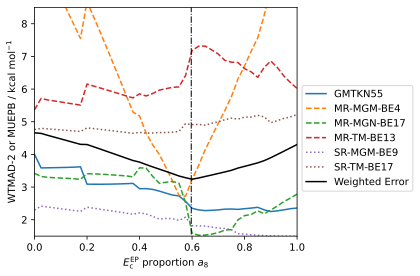
\includegraphics[width=0.6\textwidth]{assets/plot-seq-cr-proportion.pdf}
  \caption{XYG6+1/cr 在限制参数 $a_8$ 下对加权误差的拟合后数据集误差表现。}
  \label{fig.2.plot-seq-cr-proportion}
\end{figure}

首先考虑 IEPA-like 相关能的引入。这里以 XYG6+1/cr 模型为例。图 \ref{fig.2.plot-seq-cr-proportion} 展示的是限制 $E_\mathrm{c}^\text{MP2/cr}$ 在 $E_\mathrm{c}^\mathrm{PT}$ 效应中的占比数 $a_8$ 时,各数据子集误差随 $a_8$ 取值的变化情况。特别地,当取 $a_8 = 0$ (图像最右侧) 时,该模型化归为 XYG6 模型;当取 $a_8 = 1$ (图像最左侧) 时,该模型的微扰相关能完全是 MP2/cr;点划线表示加权误差取到最小时参数 $a_8$ 的数值,即 \ref{sec.2.xyg6-1-model-benchmark} 小节中所定义的 XYG6+1/cr 近似泛函。

受参数 $a_8$ 影响最大的数据集是 MR-MGM-BE4 (多参考主族金属键解离能);若不引入 ($a_8 = 0$) 或完全引入 ($a_8 = 1$) $E_\mathrm{c}^\mathrm{MP2/cr}$ 相关能,其 MUEPB 误差都将超过 8 \si{kcal.mol^{-1}}。事实上,从附录的表 \ref{tab.2.supp.MR-MGM-BE4} 中可以看到,XYG$n$ ($n=3,6,7$) 在 MR-MGM-BE4 测评中,阴离子 \ce{KO-} 与 \ce{LiO-} 的误差很大;其误差分别在 40 \si{kcal.mol^{-1}} 与 20 \si{kcal.mol^{-1}} 左右。这两个体系具有 1 eV 的小 HOMO/LUMO gap,因此可以预期到仅使用 MP2 相关能的 XYG$n$ ($n=3,6,7$) 在这类体系上表现较差。当 $a_8 \simeq 0.6$ 时,MP2/cr 的引入有效地缓解了这两个离子的误差到小于 10 \si{kcal.mol^{-1}},从而 MR-MGM-BE4 子集的 MUEPB 整体误差降至 3 \si{kcal.mol^{-1}} 左右。

对于其它数据集,一般来说,参数 $a_8$ 越大,越有利于 GMTKN55 数据集与 SR-MGM-BE9 子集的误差下降,尽管下降幅度较小;$a_8$ 对于 SR-TM-BE17 数据集的影响不大。需要指出的是,对于 $a_8 \simeq 0.6$ 的情形 (如表 \ref{tab.2.supp.SR-TM-BE17} 所示),SR-TM-BE17 数据集的 \ce{Zr2} 体系 HOMO/LUMO gap 是较小的 1.34 eV,处于 IEPA-like 相关能可以对 MP2 相关能产生有效矫正的范围;在引入 IEPA-like 相关能后计算误差相对于 XYG$n$ ($n=3,6,7$) 下降约 20 \si{kcal.mol^{-1}}。但同时因为其它计算体系的误差有小幅上升,因此 SR-MGM-BE9 子集的整体误差没有下降太多。

值得注意的是 MR-TM-BE13 与 MR-MGN-BE17 的表现在 XYG6+1/cr 模型下 $a_8 = 0.6$ 附近有较大的跳变;这个跳变的影响因素比较可能是间接地因参数优化过程中 $c_\mathrm{x} = a_1$ 即严格交换能的占比跳变较大有关,如图 \ref{fig.2.plot-seq-cr-against-cx} 所示。可以发现,MR-TM-BE13 数据集的 MUEPB 误差通常随严格交换系数 $c_\mathrm{x}$ 的增大而增大;相反地,MR-MGN-BE17 的 MUEPB 误差则随 $c_\mathrm{x}$ 的增大而减小。因此,该误差跳变不能简单地归因于 MP2/cr 的引入本身。关于严格交换能占比参数 $c_\mathrm{x}$ 对各数据集的影响,将在后一小节 \ref{sec.2.proportion-exchange} 中阐述。

\begin{figure}[h]
  \centering
  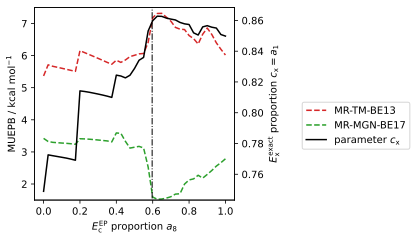
\includegraphics[width=0.6\textwidth]{assets/plot-seq-cr-against-cx.pdf}
  \caption{XYG6+1/cr 在限制参数 $a_8$ 下对加权误差的拟合后 MR-TM-BE13、MR-MGN-BE17 数据集的 MUEPB 误差表现、以及参数 $c_\mathrm{x} = a_1$ 在给定参数 $a_8$ 下的变化情况。}
  \label{fig.2.plot-seq-cr-against-cx}
\end{figure}

在这一小节的最后,我们考察引入 IEPA-like 相关能后表现较差的体系。以 XYG6+1/cr 近似泛函为例,MR-TM-BE13 子集 (表 \ref{tab.2.supp.MR-TM-BE13}) 中的 \ce{TiCl}、\ce{NiCH2+}、\ce{VO} 以及 SR-TM-BE17 子集 (表 \ref{tab.2.supp.SR-TM-BE17}) 中的 \ce{CoH}、\ce{FeH}、\ce{FeCl},这些体系平均每个键的解离误差大于 10 \si{kcal.mol^{-1}}。由于这些体系的 HOMO/LUMO gap 均大于 1.5 eV,因此 MP2/cr 相关能与 MP2 相关能表现上会比较接近,从而难以通过仅引入 MP2/cr 相关能解决这类体系的计算误差。

\subsection{参数优化讨论:严格交换能占比}
\label{sec.2.proportion-exchange}

其次考察严格交换能的占比对数据集测评的影响。图 \ref{fig.2.plot-seq} 展示的是限制严格相关能 $E_\mathrm{x}^\text{exact}$ 在总交换能中的占比数 $c_\mathrm{x} = a_1$ 时,各数据子集误差随 $c_\mathrm{x}$ 取值的变化情况。

首先,从上一小节 \ref{sec.2.proportion-iepa-like} 的讨论中,我们已经注意到 IEPA-like 相关能的引入对 MR-MGM-BE4 子集的 MUEPB 测评表现、特别是 \ce{KO-} 与 \ce{LiO-} 离子的解离能有很大的提升;在图 \ref{fig.2.plot-seq} 中,可以清晰地看到在 $c_\mathrm{x} > 0.5$ 时,XYG6+1 参数模型在 MR-MGM-BE4 的测评结果上明显优于没有引入 IEPA-like 相关能的 XYG$n$ ($n=6,7$)。同时,对于 XYG6+1/cr 模型,其 GMTKN55、MR-MGN-BE17 与 MR-TM-BE13 在 $c_\mathrm{x} > 0.5$ 时的误差相较于 XYG$n$ ($n=6,7$) 有一定提升,SR-MGM-BE9 与 SR-TM-BE17 的误差与 XYG$n$ ($n=6,7$) 接近;考虑到一般的双杂化泛函近似都选用 $c_\mathrm{x} > 0.5$,因此图 \ref{fig.2.plot-seq} 的结果进一步验证了引入 IEPA-like、特别是 MP2/cr 相关能,对整体误差表现确实有所提升。

但对于其它数据集而言,不论选取哪一种模型,总体上
\begin{itemize}[nosep]
  \item $c_\mathrm{x}$ 愈接近 0.9,GMTKN55 数据集的 WTMAD-2 误差愈小;
  \item $c_\mathrm{x}$ 愈接近 0.5,MR-TM-BE13 子集的 MUEPB 误差愈小;
  \item SR-TM-BE17 子集的误差比较平稳,在 $c_\mathrm{x}$ 取 0.7 时通常较小。
\end{itemize}
考虑到 GMTKN55 数据集在拟合过程中的权重较大、MR-TM-BE13 与 MR-MGM-BE4 子集的误差本身较大,且这三个数据集误差对 $c_\mathrm{x}$ 的变化比较敏感,因此对泛函模型进行参数优化时,$c_\mathrm{x}$ 取值事实上平衡这三个数据集的误差。由于 IEPA-like 相关能的引入大幅降低了 MR-MGM-BE4 的误差、并一定程度地降低了 MR-TM-BE13 的误差以及其对 $c_\mathrm{x}$ 取值的敏感程度,因此 XYG6+1 模型所优化得到的参数中 $c_\mathrm{x}$ 取值比较接近 GMTKN55 数据集下表现良好的范围即 $c_\mathrm{x} \simeq 0.9$。而对于 XYG$n$ ($n=6,7$) 模型而言,降低参数 $c_\mathrm{x}$ 可以在牺牲一定的 GMTKN55 误差时显著降低 MR-TM-BE13 与 MR-MGM-BE4 的误差,因此参数这类模型倾向于优化 $c_\mathrm{x}$ 到大约 0.7 左右。

\begin{figure}[h]
  \centering
  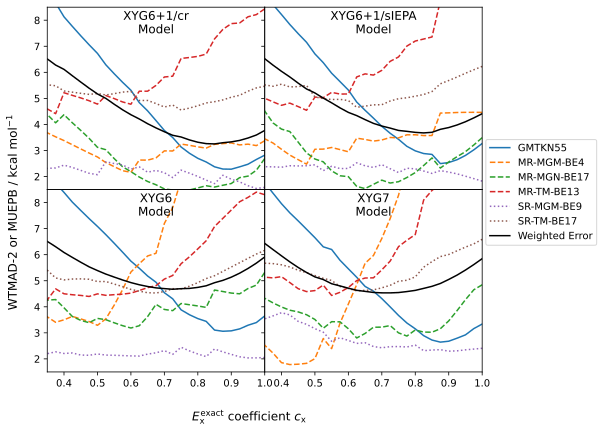
\includegraphics[width=0.9\textwidth]{assets/plot-seq.pdf}
  \caption{诸参数模型在限制参数 $c_\mathrm{x} = a_1$ 下对加权误差的拟合后数据集的误差表现。}
  \label{fig.2.plot-seq}
\end{figure}

Yu 等\cite{Yu-Truhlar.CS.2016} 认为,Hartree-Fock 交换能通常可以提升碳水化合物、弱相互作用、反应能垒等问题上有较好的表现 (这些也是 GMTKN55 数据集着重关心的问题),但会破坏多参考体系问题的表现。尽管 Yu 等的主张是针对杂化泛函所提,但图 \ref{fig.2.plot-seq} 表明在 $c_\mathrm{x} > 0.5$ 的情形下表明基于 B3LYP 轨道的双杂化泛函也有相同的结论。

XYG6+1 模型尽管对以 \ce{KO-}、\ce{LiO-}、\ce{Zr2} 为代表的 HOMO/LUMO gap 较小的计算问题有更好的处理,但需要指出的是,尽管引入了 IEPA-like 型相关能的 XYG6+1 模型一定程度上减少了 MR-TM-BE13 的误差,但减小幅度远小于降低 $c_\mathrm{x}$ 所带来的收益;类如 \ce{TiCl}、\ce{NiCH2+}、\ce{VO}、\ce{CoH}、\ce{FeH}、\ce{FeCl} 等困难的计算问题,一定程度地降低 $c_\mathrm{x}$ 尽管能有更好的计算表现,但同时会推高 GMTKN55 为代表的主族化学问题的误差。因此需要承认,为要更好地解决这两类问题,仅使用引入 IEPA-like 相关能的 XYG6+1 框架仍然是不够的。

\subsection{参数优化讨论:数据集的影响}
\label{sec.2.propotion-dataset}

简单讨论引入 Minnesota 2015 数据集与否,对参数优化结果的影响。图 \ref{fig.2.plot-seq-xyg7} 展示了 XYG6+1/cr 模型下,仅对 GMTKN55 数据集参数优化、与额外引入 Minnesota 2015 五个数据子集参数优化的误差比较。可以看到,引入额外的数据集、并重新定义误差量标,确实会使得部分数据子集的误差表现有明显的变化。引入 Minnesota 2015 数据集进行优化后,在所有图中展示的 $c_\mathrm{x}$ 区域内对 GMTKN55 的 WTMAD-2 误差量标有大约 0.5 \si{kcal.mol^{-1}} 的增加。因此,GMTKN55 的误差总体变化不大;由于我们在构造加权误差时对 GMTKN55 的 WTMAD-2 施加权重为很大的 48\%,因此 GMTKN55 的误差变化较小是可以预期的。

当 Minnesota 2015 五个数据子集纳入拟合集时,尽管每个子集分到的权重不超过 12\%,但除 SR-MGM-BE9 外的数据子集误差显著下降;SR-MGM-BE9 的误差在 $c_\mathrm{x} > 0.5$ 的范围内也可以控制在 3 \si{kcal.mol^{-1}} 以内。这意味着,从积极的角度来看,即使参数拟合没有严重地偏向于每一个参与加权误差计算的 Minnesota 2015 数据子集,XYG6+1/cr 模型也能在不严重影响 GMTKN55 误差的前提下,较好地改善这些子集的表现,从而在更广泛的化学问题上有优异的表现。但从消极的角度看,也意味着在当前的加权误差标准下,这些 Minnesota 2015 子集的误差对 XYG6+1/cr 模型的参数并不是非常稳健;若对加权误差的表达式作较大程度的改变、或引入其它数据集参与参数拟合,这些子集的误差有很大可能会被较大程度地改变。

同时需要注意到,若没有引入 Minnesota 2015 数据子集、而仅以 GMTKN55 数据集进行拟合时,XYG6+1/cr 模型对这五个数据子集 (如图 \ref{fig.2.plot-seq-xyg7} 左侧所示) 的预测表现不能称为良好。若以此现象外推,则不能期望 \ref{sec.2.xyg6-1-model-benchmark} 小节所提出的 XYG6+1/cr 近似泛函可以以与 GMTKN55 和 Minnesota 2015 五个数据子集相同的精度解决被拟合的数据集以外的化学问题。这部分的讨论对除 MP2/cr 以外的其它掺杂 IEPA-like 相关能的 XYG6+1 参数模型泛函同样适用。

\begin{figure}[h]
  \centering
  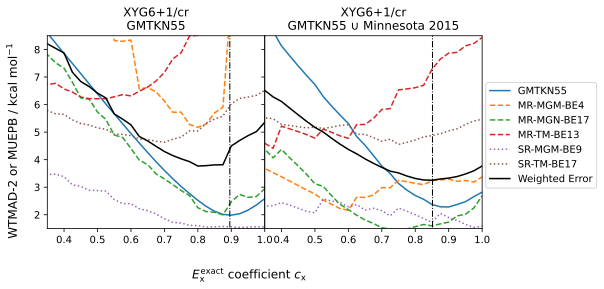
\includegraphics[width=0.9\textwidth]{assets/plot-seq-cr.pdf}
  \caption{XYG6+1/cr 模型在限制参数 $c_\mathrm{x} = a_1$ 下对数据集拟合后数据集的误差表现。\\左图针对 GMTKN55 的 WTMAD-2 误差量标优化,右图针对 GMTKN55 与 Minnesota 2015 五个子集的加权误差量标优化。点划线表示在对应误差量标下 $c_\mathrm{x}$ 的最佳取值。}
  \label{fig.2.plot-seq-xyg7}
\end{figure}

\subsection{XYG6+1 模型泛函在分子解离曲线问题的表现}

在本节最后,将简短地考察 XYG6+1 模型泛函的在部分分子解离曲线问题的表现。

作为三键体系,\ce{N2} 氮气解离问题是最有挑战性的分子解离势能面问题之一。在图 \ref{fig.2.curve-N2} 中可以看到,在解离曲线 1.0--2.0 \AA 的范围内,XYG6+1/cr 方法与 DMC 方法之间的误差普遍在 30 \si{kcal.mol^{-1}} 以内;而 XYG6+1/IEPA 方法与 CCSD(T)、DMC 方法的结果在 1.0--2.0 \AA 非常接近。XYG6+1/sIEPA 尽管存在较大误差,但相较于 MP2、MP2/cr-III、XYG$n$ ($n=3,7$) 等方法,在键长超过 1.4 \AA 时严重下行的趋势上有所改善。

但需要指出,在图中所测评的基于单参考态的近似方法中,几乎没有可以正确预言超过 2.0 \AA 后解离的趋势。CCSD 方法尽管在解离后段趋于准确值 (两个氮原子的能量和),但由于在 1.0--2.0 \AA 区间高估了解离趋势,因此产生了非物理的凸包。CCSD(T) 与 XYG6+1/cr 方法尽管在 1.0--2.0 \AA 的范围内表现良好,但在 2.0 \AA 以后的区域有明显下行趋势。XYG6+1/sIEPA 与 XYG6+1/IEPA 方法则在 2.0 \AA 以后的区域有明显的上行趋势;这是因为尽管 sIEPA 与 IEPA 相关能的趋势是下行,但 MP2 相关能相比于 sIEPA 与 IEPA 相关能下行趋势要明显地多;而 XYG6+1/sIEPA 与 XYG6+1/IEPA 的 MP2 在总微扰型相关能中的占比分别约为 -0.42\% 和 -0.11\%,由于 MP2 相关能负系数的原因,XYG6+1/sIEPA 与 XYG6+1/IEPA 显现出了与 MP2 相反的上升趋势。由于 XYG6+1/sIEPA 中 MP2 相关能的负系数占比更大,因此 XYG6+1/sIEPA 比 XYG6+1/IEPA 更早、更明显地在势能面上显现出错误的上升趋势。

\begin{figure}[h]
  \centering
  \includegraphics[width=0.7\textwidth]{assets/curve-N2.pdf}
  \caption{各方法在 \ce{N2} 解离曲线的表现。}
  \label{fig.2.curve-N2}
\end{figure}

随后考虑 \ce{F2} 解离曲线。在图 \ref{fig.2.curve-F2} 中,仍然没有方法能完全正确地预言合理的解离趋势。尽管 CCSD(T) 的 \ce{F2} 解离曲线在 1.2 \AA 后始终是倾向于成键的 (势能面的能量在 0 \si{kcal.mol^{-1}} 以下),但在 2.2 \AA 以后显现出不正确的下行趋势。XYG6+1/cr、XYG6+1/sIEPA 与 XYG$n$ (n=3,7) 在 1.2--1.6 \AA 的成键区域中,能量与 CCSD(T) 非常接近。但在 2.0 \AA 后的区域中,XYG$n$ ($n=3,7$) 有着比 CCSD(T) 更加严重的下行。相反地,诸 XYG6+1 近似泛函与 CCSD、B3LYP、MP2/cr-III 等方法则在成键区域以后严重高估势能面;这些方法在 1.6--2.0 \AA 的区域中有比较接近的数值。

\begin{figure}[h]
  \centering
  \includegraphics[width=0.7\textwidth]{assets/curve-F2.pdf}
  \caption{各方法在 \ce{F2} 解离曲线的表现。}
  \label{fig.2.curve-F2}
\end{figure}

\ce{H2O} 与 \ce{F2} 体系同样是单键解离问题。从图 \ref{fig.2.curve-H2O} 与图 \ref{fig.2.curve-H2O-part} 中可以看出,相比于 \ce{F2},各方法在 \ce{H2O} 体系上的表现明显普遍较好,但仍然存在一些问题。CCSD(T)、XYG3 方法在 2.0 \AA 以前与 DMC 的结果非常接近,但 2.0 \AA 以后显现出下降的趋势。XYG7 在解离曲线后期普遍低估能量。除 CCSD(T)、XYG$n$ ($n=3, 7$) 外的方法则对解离曲线有一定程度的高估;其中 MP2 与 XYG6+1/sIEPA 方法在 1.4--1.8 \AA 与作为参考值的 DMC 结果非常接近、其它方法则在这一段解离曲线上也稍有误差。

\begin{figure}[h]
  \centering
  \includegraphics[width=0.7\textwidth]{assets/curve-H2O.pdf}
  \caption{各方法在 \ce{H2O} 解离曲线的表现。}
  \label{fig.2.curve-H2O}
\end{figure}

\begin{figure}[h]
  \centering
  \includegraphics[width=0.7\textwidth]{assets/curve-H2O-part.pdf}
  \caption{各方法在 \ce{H2O} 解离曲线 1.4--2.25 \AA 段的表现。}
  \label{fig.2.curve-H2O-part}
\end{figure}

作为一种不太常规的单键解离问题,图 \ref{fig.2.curve-H6} 所示的环状 \ce{H6} 解离曲线也有一定挑战性。对于 CCSD 与 CCSD(T) 方法,它们在 1.8 \AA 以前的表现骄傲好,但在 2.0 \AA 以后能量明显地出现了不符合物理直觉的下降。MP2 与 MP2/cr-III 方法则不管是在 0.75--1.25 \AA 的成键区域、还是以后的解离区域,相比于参考值 DMC 都有一定程度的高估。B3LYP 在成键区域低估、但在解离区域则明显高估势能面上的能量。对于经测评的 xDH 型泛函,他们都在成键区域有良好的表现,但在解离区域产生明显的高估。

\begin{figure}[h]
  \centering
  \includegraphics[width=0.7\textwidth]{assets/curve-H6.pdf}
  \caption{各方法在 \ce{H6} 解离曲线的表现。}
  \label{fig.2.curve-H6}
\end{figure}

从上述的讨论中,我们看到大多数情形下,xDH 型泛函和 CCSD、CCSD(T) 方法在成键区域的势能面与参考值非常接近。但即使是计算化学中普遍受到认可的高精度 CCSD 与 CCSD(T) 方法,在闭壳层的限制下,也难以给出定性上正确的解离曲线;而对于其它 post-HF 与密度泛函近似方法更是如此。引入 IEPA 类型相关能的诸 XYG6+1 模型可以在 \ce{N2} 问题上,相较于 XYG$n$ ($n=3,7$) 有很大程度的改善,成功地避免了解离过程中段过于严重的负误差;但正因为一般来说 IEPA 型相关能绝对值小于 MP2 相关能、并且 HOMO/LUMO gap 愈小 IEPA 型相关能与 MP2 相关能之间的差距愈大,因此绝大多数情况下诸多 XYG6+1 模型近似泛函的势能面比 XYG$n$ 模型要高。对于所有经测评的单键解离体系,相比于 DMC 参考值、或者解离极限的原子能量之和而言,XYG$n$ ($n=3,7$) 的势能面在解离区域已经有较大程度的高估;在这种情况下,正因为引入了 IEPA 型相关能,XYG6+1 模型实际上会更严重地高估势能面。因此,我们无法给出简单的结论,表明 XYG6+1 模型是否在解离曲线问题上,相比于 XYG$n$ ($n=3,7$) 是否有改善。

\section{本章小结}

在本章工作中,我们简单回顾了作为双杂化泛函理论基础的 G\"orling-Levy 微扰理论。该理论联系起 post-HF 方法与密度泛函近似。作为该微扰理论的近似,GLPT2 是诸多双杂化泛函的理论基础。GLPT2 一般由 MP2 相关能实现,而 MP2 相关能在 HOMO/LUMO gap 较小时存在明显的负误差。籍此,我们简单回顾了 IEPA 理论,并表明这些 IEPA 型相关能可以缓解 MP2 相关能在 HOMO/LUMO gap 较小情况下的误差。类似于 post-HF 框架之于 IEPA 的关系,我们对 G\"orling-Levy 微扰框架下引入 IEPA 型相关能的理论合理性作了说明。

为缓解基于 MP2 型相关能的双杂化泛函在以 \ce{N2} 解离、含过渡金属体系为代表的 HOMO/LUMO gap 较小体系上存在一定负误差的情况,同时保证在以主族反应势垒、键解离能、弱相互作用能为代表的、主流双杂化泛函表现较好的问题上保持较小的误差,我们尝试在 GMTKN55 数据集上有优异表现的 xDH@B3LYP 框架下引入 IEPA 型相关能以构造新的 XYG6+1 参数模型。在参数优化上,除了着重主族化学的 GMTKN55 外,我们引入部分含有多参考信息与过渡金属信息的 Minnesota 2015 子数据集,作参数优化得到新的泛函近似;它们依引入的相关能形式不同,称为 XYG6+1/cr、XYG6+1/IEPA 与 XYG6+1/sIEPA。

参数优化与测评结果表明,XYG6+1/cr 近似泛函在各个数据集上的表现有良好的平衡。对于 \ce{KO-}、\ce{LiO-}、\ce{Zr2} 等 HOMO/LUMO gap 小于 1.5 eV 的体系,键解离能的计算误差从 20--40 \si{kcal.mol^{-1}} 降到 10 \si{kcal.mol^{-1}} 以下,有效地降低了这类体系误差。同时,XYG6+1/cr 在 GMTKN55 数据集上的总体 WTMAD-2 误差为 2.36 \si{kcal.mol^{-1}},其表现相比于目前流行的 MP2 型相关能的双杂化泛函仍然良好;在我们所定义的 GMTKN55 和 Minnesota 2015 部分子数据集上的加权误差为 3.28 \si{kcal.mol^{-1}},是表现最优异的泛函。XYG6+1/cr 很好地平衡了主族化学问题与多参考特性或过渡金属问题的误差,基本达到了设计该泛函近似的初衷。XYG6+1/sIEPA 泛函也有类似的良好表现。

但需要承认,仅引入 IEPA 型相关能、并作关于 GMTKN55 和 Minnesota 2015 部分子数据集的优化得到的泛函,仍然存在着困难。
\begin{itemize}[nosep]
  \item 首先,HOMO/LUMO gap 小的体系一般具有多参考特性,但多参考特性的体系 HOMO/LUMO gap 不一定小;在诸如 \ce{TiCl}、\ce{NiCH2+}、\ce{VO} 为代表的多参考特性的体系上,XYG6+1 模型泛函表现较差。此外,诸如 \ce{CoH}、\ce{FeH}、\ce{FeCl} 等单参考特性含过渡金属体系的键解离也存在较大误差,而多参考特性的 MR-MGN-BE17 数据集的总的误差相当低,表明 XYG6+1 模型的误差来源与单参考或多参考的关联性不一定很强,而可能与过渡金属本身关联性稍大。
  \item 在分子解离曲线问题上,在闭壳层限制下,尽管 XYG6+1 参数模型在 \ce{N2} 体系上 2.0 \AA 以前的表现较好,但仍然无法避免解离到更远时定性不正确的趋势;而在以 \ce{F2}、\ce{H2O}、环状 \ce{H6} 为代表的单键解离问题上,不论是否引入 IEPA 或 MP2 型相关能,都在解离区域存在较大的正误差。这意味着在密度泛函近似中,仅仅矫正 MP2 相关能在 HOMO/LUMO gap 较小时的误差表现,不足以漂亮地解决解离曲线的问题。
  \item 对参数优化过程的讨论,表明严格交换能 $E_\mathrm{x}^\mathrm{exact}$ 占比愈大对 GMTKN55 主族化学问题的误差愈小、但相应地 MR-TM-BE13 等含过渡金属或多参考特性体系的数据集误差愈大;这个现象并不因为在泛函中引入 IEPA 型相关能而有所改善。同时,对于 XYG6+1 参数模型优化得到的泛函,误差容易随参与拟合数据集的变化而波动,表明该参数模型下的泛函不是非常稳健。我们无法建议将 XYG6+1 参数模型下优化的泛函,应用在 GMTKN55 与 Minnesota 2015 五个子数据集的目标化学问题以外的体系计算上。
\end{itemize}

\clearpage

\section{附录:补充数据}

\begin{table}[ht]
\centering
\caption{部分 xDH@B3LYP 模型与 XYG6+1 模型近似泛函在 MR-MGM-BE4 子集上误差。\\反应能与 MUEPB 单位 \si{kcal.mol^{-1}};HOMO/LUMO gap 单位 eV。}
\label{tab.2.supp.MR-MGM-BE4}
\widetabular{
  \begin{tabular}{ld{1.2}d{3.2}d{3.2}d{3.2}d{3.2}d{3.2}d{3.2}}
  \toprule
  \multicolumn{2}{c}{MR-MGM-BE4} & \multicolumn{3}{c}{xDH@B3LYP} & \multicolumn{3}{c}{XYG6+1\tnote{a}} \\
  \cmidrule(lr){1-2} \cmidrule(lr){3-5} \cmidrule(lr){6-8}
  体系 & \multicolumn{1}{c}{gap} & 
  \multicolumn{1}{c}{XYG3} & \multicolumn{1}{c}{XYG6} & \multicolumn{1}{c}{XYG7} &
  \multicolumn{1}{c}{MP2/cr} & \multicolumn{1}{c}{sIEPA} & \multicolumn{1}{c}{IEPA} \\
  \midrule
  \ce{CaO } & 2.54 & 7.01  & 8.03  & 1.50  & 1.41      & 0.18         & 0.68        \\
  \ce{KO- } & 1.03 & 38.03 & 56.57 & 46.24 & 0.00      & 0.00         & 0.00        \\
  \ce{LiO-} & 1.03 & 19.40 & 25.28 & 20.65 & 5.80      & 9.54         & 3.99        \\
  \ce{MgS } & 1.75 & -3.27 & -1.52 & -2.83 & -5.75     & -4.77        & -5.81       \\
  \midrule
  MUEPB     &      & 16.93 & 22.85 & 17.81 & 3.24      & 3.62         & 2.62        \\
  \bottomrule
  \end{tabular}
}{
  \item[a] 为方便排版,表头第二行指代的是 XYG6+1 模型泛函所使用的 IEPA 型相关能 $E_\mathrm{c}^\text{IEPA-like}$ 的具体类型;即 MP2/cr 指代 XYG6+1/cr、sIEPA 指代 XYG6+1/sIEPA、IEPA 指代 XYG6+1/IEPA。后续表格类同。
}
\end{table}

\begin{table}[ht]
\centering
\caption{部分 xDH@B3LYP 模型与 XYG6+1 模型近似泛函在 MR-MGN-BE17 子集上误差。\\反应能与 MUEPB 单位 \si{kcal.mol^{-1}};HOMO/LUMO gap 单位 eV。}
\label{tab.2.supp.MR-MGN-BE17}
\widetabular{
  \begin{tabular}{ld{2.2}d{3.2}d{3.2}d{3.2}d{3.2}d{3.2}d{3.2}}
  \toprule
  \multicolumn{2}{c}{MR-MGN-BE17} & \multicolumn{3}{c}{xDH@B3LYP} & \multicolumn{3}{c}{XYG6+1} \\
  \cmidrule(lr){1-2} \cmidrule(lr){3-5} \cmidrule(lr){6-8}
  体系\tnote{a} & \multicolumn{1}{c}{gap\tnote{b}} & 
  \multicolumn{1}{c}{XYG3} & \multicolumn{1}{c}{XYG6} & \multicolumn{1}{c}{XYG7} &
  \multicolumn{1}{c}{MP2/cr} & \multicolumn{1}{c}{sIEPA} & \multicolumn{1}{c}{IEPA} \\
  \midrule
  \ce{NF3 }          &  10.08 & -2.57 & -0.70 & -1.54 & -0.60     & -0.89        & -1.13       \\
  \ce{CO2 }          &  9.87  & -0.40 & 1.84  & -0.25 & 0.61      & 0.42         & -0.12       \\
  \ce{SiO }          &  6.34  & 1.65  & 3.88  & 1.26  & -0.22     & 0.00         & -2.69       \\
  \ce{SO2 }          &  5.69  & -1.34 & 1.50  & -0.71 & -0.84     & -0.99        & -2.35       \\
  \ce{CO2 }          &  9.41  & -1.06 & 1.84  & -0.11 & -0.25     & 0.10         & -2.29       \\
  \ce{SO2 }          &  3.69  & 0.29  & 0.41  & -0.87 & -1.46     & -3.63        & -1.81       \\
  \ce{ClO }          &  2.78  & -1.94 & -0.71 & -1.48 & -1.95     & -3.02        & -2.43       \\
  \ce{F2  }          &  7.23  & -6.91 & -2.23 & -4.17 & -3.35     & -3.28        & -6.35       \\
  \ce{N2  }          &  10.99 & 1.17  & 2.60  & 2.31  & -1.35     & 1.97         & -3.23       \\
  \ce{O2  }          &  5.28  & -1.09 & -1.29 & -1.67 & -2.65     & -7.06        & -3.60       \\
  \ce{NO  }          &  3.01  & -0.43 & 1.33  & 0.77  & -1.27     & -0.43        & -3.02       \\
  \ce{CN  }          &  3.58  & 2.82  & 5.52  & 3.05  & -0.28     & 0.89         & -3.54       \\
  \ce{B2  }          &  2.17  & -1.12 & 2.16  & -0.67 & -5.74     & -9.10        & -7.72       \\
  \ce{O3  }\tnote{c} &  4.12  & 0.30  & 13.49 & 8.35  & 0.06      & 3.59         & -7.78       \\
  \ce{C2  }          &  1.80  & 4.19  & 17.97 & 10.48 & -5.59     & -2.42        & -15.25      \\
  \ce{S4  }\tnote{d} &  2.28  & 1.56  & 9.44  & 6.47  & -1.59     & 2.84         & -2.51       \\
  \ce{Cl2O}\tnote{e} &  4.31  & -1.98 & 0.60  & -0.61 & -0.29     & -0.45        & -1.64       \\
  \midrule
  MUEPB              &        & 1.81  & 3.97  & 2.63  & 1.65      & 2.42         & 3.97        \\
  \bottomrule
  \end{tabular}
}{
  \item[a] 对于未标明化学反应式的体系,其对应的反应是原子化反应。后续表格类同。
  \item[b] 对于开壳层体系,HOMO/LUMO gap 是通过 $\alpha, \beta$ 两种自旋的 HOMO 最大值与 LUMO 最小值的差减计算得到。后续表格类同。
  \item[c] \ce{O3 -> O2 + O}
  \item[d] \ce{S4 -> 2 S2}
  \item[e] \ce{Cl2O -> Cl2 + O}
}
\end{table}

\begin{table}[ht]
\centering
\caption{部分 xDH@B3LYP 模型与 XYG6+1 模型近似泛函在 MR-TM-BE13 子集上误差。\\反应能与 MUEPB 单位 \si{kcal.mol^{-1}};HOMO/LUMO gap 单位 eV。}
\label{tab.2.supp.MR-TM-BE13}
\widetabular{
  \begin{tabular}{ld{1.2}d{3.2}d{3.2}d{3.2}d{3.2}d{3.2}d{3.2}}
  \toprule
  \multicolumn{2}{c}{MR-TM-BE13} & \multicolumn{3}{c}{xDH@B3LYP} & \multicolumn{3}{c}{XYG6+1} \\
  \cmidrule(lr){1-2} \cmidrule(lr){3-5} \cmidrule(lr){6-8}
  体系 & \multicolumn{1}{c}{gap} & 
  \multicolumn{1}{c}{XYG3} & \multicolumn{1}{c}{XYG6} & \multicolumn{1}{c}{XYG7} &
  \multicolumn{1}{c}{MP2/cr} & \multicolumn{1}{c}{sIEPA} & \multicolumn{1}{c}{IEPA} \\
  \midrule
  \ce{TiCl    }          & 5.72 & -10.78 & -13.28 & -15.27 & -12.64    & -18.46       & -10.47      \\
  \ce{VF5     }          & 5.94 & 5.37   & 9.00   & 6.49   & 5.15      & 3.76         & 0.96        \\
  \ce{CrCl    }          & 2.93 & 3.09   & 3.13   & 3.18   & 1.10      & 2.35         & 0.69        \\
  \ce{CrOF    }          & 1.68 & -5.09  & 0.04   & -3.31  & -6.61     & -4.28        & -11.81      \\
  \ce{(FeBr2)2}          & 2.73 & 8.23   & 9.72   & 10.04  & 8.49      & 8.91         & 8.22        \\
  \ce{Co(CO)4H}          & 5.89 & 20.39  & 27.69  & 23.02  & 13.45     & 13.98        & 8.34        \\
  \ce{NiCH2+  }\tnote{a} & 3.90 & 18.44  & 20.94  & 18.52  & 12.16     & 8.34         & 8.73        \\
  \ce{FeCO5   }\tnote{b} & 4.96 & 24.37  & 29.99  & 26.32  & 12.90     & 15.84        & 11.56       \\
  \ce{VS      }          & 2.90 & 14.57  & 17.19  & 15.79  & 3.69      & 3.25         & -0.99       \\
  \ce{CuCl    }          & 3.99 & 1.28   & 3.15   & 2.59   & 1.21      & 1.81         & 0.75        \\
  \ce{CuH     }          & 4.23 & 2.29   & 2.91   & 3.57   & 0.97      & 2.20         & 0.33        \\
  \ce{NiCl    }          & 3.14 & 4.75   & 6.76   & 5.81   & 4.17      & 4.08         & 2.89        \\
  \ce{VO      }          & 2.55 & 20.04  & 27.78  & 23.64  & 13.58     & 13.49        & 3.22        \\
  \midrule
  MUEPB                  &      & 10.67  & 13.20  & 12.12  & 7.40      & 7.75         & 5.30        \\
  \bottomrule
  \end{tabular}
}{
  \item[a] \ce{NiCH2+ -> Ni+ + CH2}
  \item[b] \ce{FeCO5 -> Fe + 5CO}
}
\end{table}

\begin{table}[ht]
\centering
\caption{部分 xDH@B3LYP 模型与 XYG6+1 模型近似泛函在 SR-MGM-BE9 子集上误差。\\反应能与 MUEPB 单位 \si{kcal.mol^{-1}};HOMO/LUMO gap 单位 eV。}
\label{tab.2.supp.SR-MGM-BE9}
\widetabular{
  \begin{tabular}{ld{1.2}d{3.2}d{3.2}d{3.2}d{3.2}d{3.2}d{3.2}}
  \toprule
  \multicolumn{2}{c}{SR-MGM-BE9} & \multicolumn{3}{c}{xDH@B3LYP} & \multicolumn{3}{c}{XYG6+1} \\
  \cmidrule(lr){1-2} \cmidrule(lr){3-5} \cmidrule(lr){6-8}
  体系 & \multicolumn{1}{c}{gap} & 
                 \multicolumn{1}{c}{XYG3} & \multicolumn{1}{c}{XYG6} & \multicolumn{1}{c}{XYG7} &
                 \multicolumn{1}{c}{MP2/cr} & \multicolumn{1}{c}{sIEPA} & \multicolumn{1}{c}{IEPA} \\
  \midrule
  \ce{AlCl3}          & 7.35 & 0.02  & 0.72  & -0.07 & -0.11     & 0.29         & 0.55        \\
  \ce{AlF3 }          & 9.43 & -1.23 & -0.30 & -3.03 & -0.74     & -1.39        & -1.18       \\
  \ce{KOH  }\tnote{a} & 3.72 & -1.73 & -0.79 & -3.14 & -2.71     & -2.55        & -3.59       \\
  \ce{NaO  }          & 3.09 & -2.18 & -2.62 & -4.22 & -4.25     & -3.79        & -4.47       \\
  \ce{LiO  }          & 3.41 & 1.83  & 0.52  & -0.92 & -0.72     & -0.12        & -0.03       \\
  \ce{LiCl }          & 5.31 & -0.87 & -1.58 & -2.43 & -2.99     & -2.17        & -2.00       \\
  \ce{AlCl3}          & 5.01 & -0.05 & 0.39  & -0.26 & -0.81     & -0.39        & -0.32       \\
  \ce{ZnSe }          & 1.64 & 6.16  & 7.86  & 7.89  & 4.51      & 5.43         & 4.55        \\
  \ce{ZnCl }          & 2.34 & 0.25  & 1.22  & 0.97  & 0.93      & 0.75         & 1.54        \\
  \midrule
  MUEPB              &      & 1.59  & 1.78  & 2.55  & 1.97      & 1.87         & 2.03        \\
  \bottomrule
  \end{tabular}
}{
  \item[a] \ce{KOH -> K + OH}
}
\end{table}

\begin{table}[ht]
\centering
\caption{部分 xDH@B3LYP 模型与 XYG6+1 模型近似泛函在 SR-TM-BE17 子集上误差。\\反应能与 MUEPB 单位 \si{kcal.mol^{-1}};HOMO/LUMO gap 单位 eV。}
\label{tab.2.supp.SR-TM-BE17}
\widetabular{
  \begin{tabular}{ld{1.2}d{3.2}d{3.2}d{3.2}d{3.2}d{3.2}d{3.2}}
  \toprule
  \multicolumn{2}{c}{SR-TM-BE17} & \multicolumn{3}{c}{xDH@B3LYP} & \multicolumn{3}{c}{XYG6+1} \\
  \cmidrule(lr){1-2} \cmidrule(lr){3-5} \cmidrule(lr){6-8}
  体系 & \multicolumn{1}{c}{gap} & 
                 \multicolumn{1}{c}{XYG3} & \multicolumn{1}{c}{XYG6} & \multicolumn{1}{c}{XYG7} &
                 \multicolumn{1}{c}{MP2/cr} & \multicolumn{1}{c}{sIEPA} & \multicolumn{1}{c}{IEPA} \\
  \midrule
  \ce{CrCl2           }          & 2.60 & 1.40  & 3.42  & 3.43  & 1.60      & 5.75         & 1.47        \\
  \ce{MnF2            }          & 5.12 & 2.27  & 3.63  & 0.51  & 3.28      & 1.43         & 1.76        \\
  \ce{FeCl2           }          & 2.93 & 5.41  & 7.02  & 7.75  & 5.57      & 6.11         & 5.36        \\
  \ce{CoCl2           }          & 3.16 & -1.54 & -0.79 & -0.27 & -2.80     & -3.80        & -2.89       \\
  \ce{Ag2             }          & 3.00 & 0.11  & 1.25  & 1.00  & -0.79     & -0.34        & -0.91       \\
  \ce{AgH             }          & 4.34 & 0.67  & 0.90  & 2.14  & -0.14     & 1.53         & 0.50        \\
  \ce{CoH             }          & 3.05 & 17.76 & 18.57 & 19.38 & 16.23     & 18.28        & 15.57       \\
  \ce{CrCH3+          }\tnote{a} & 3.49 & 3.52  & 5.06  & 5.93  & 3.78      & 5.04         & 2.89        \\
  \ce{Cu2             }          & 3.33 & -0.46 & 1.09  & 0.28  & -2.30     & -2.14        & -3.27       \\
  \ce{CuAg            }          & 3.35 & 0.10  & 1.61  & 0.89  & -0.96     & -0.84        & -1.93       \\
  \ce{CuH2O+          }\tnote{b} & 5.01 & 0.12  & 0.81  & 0.56  & 0.49      & -0.44        & 0.04        \\
  \ce{FeH             }          & 2.40 & 25.16 & 26.43 & 27.30 & 23.81     & 26.57        & 23.07       \\
  \ce{VCO+            }\tnote{c} & 2.52 & -1.99 & -4.30 & -3.33 & -4.60     & -8.32        & -3.79       \\
  \ce{Zr2             }          & 1.34 & 23.14 & 27.10 & 19.22 & 0.34      & -0.21        & -0.03       \\
  \ce{Pd(PH3)2(C6H8)  }\tnote{d} & 4.32 & 1.23  & 4.18  & 4.35  & 2.01      & 0.80         & -0.04       \\
  \ce{Pd(PH3)2(C10H12)}\tnote{e} & 4.19 & 0.29  & 4.51  & 4.62  & 1.86      & 0.21         & -1.86       \\
  \ce{FeCl            }          & 1.53 & 9.30  & 12.17 & 13.86 & 12.05     & 13.53        & 12.69       \\
  \midrule
  \ce{MUEPB           }          &      & 5.56  & 7.23  & 6.75  & 4.86      & 5.61         & 4.59        \\
  \bottomrule
  \end{tabular}
}{
  \item[a] \ce{CrCH3+ -> Cr+ + CH3}
  \item[b] \ce{CuH2O+ -> Cu+ + H2O}
  \item[c] \ce{VCO+ -> V+ + CO}
  \item[d] \ce{Pd(PH3)2(C6H8) -> Pd(PH3)2 + C6H8}
  \item[e] \ce{Pd(PH3)2(C10H12) -> Pd(PH3)2 + C10H12}
}
\end{table}

\clearpage

\begin{ThreePartTable}
\begin{longtable}{lld{2.2}d{2.2}d{2.2}d{2.2}d{2.2}d{2.2}}
  \caption{部分 xDH@B3LYP 模型与 XYG6+1 模型近似泛函在 SR-TM-BE17 子集上误差。\\小子集误差以 MAD 为量标,子集与总误差以 WTMAD-2 为量标,单位 \si{kcal.mol^{-1}}。}
  \label{tab.2.supp.GMTKN55}
  \\ \toprule
  \multicolumn{2}{c}{GMTKN55} & \multicolumn{3}{c}{xDH@B3LYP} & \multicolumn{3}{c}{XYG6+1} \\
  \cmidrule(lr){1-2} \cmidrule(lr){3-5} \cmidrule(lr){6-8}
  子集 & 小子集 & \multicolumn{1}{c}{XYG3}  & \multicolumn{1}{c}{XYG6}  & \multicolumn{1}{c}{XYG7}  & \multicolumn{1}{c}{MP2/cr} & \multicolumn{1}{c}{sIEPA} & \multicolumn{1}{c}{IEPA}  \\ \midrule
  \endfirsthead
  \caption{(续表)}
  \\ \toprule
  \multicolumn{2}{c}{GMTKN55} & \multicolumn{3}{c}{xDH@B3LYP} & \multicolumn{3}{c}{XYG6+1} \\
  \cmidrule(lr){1-2} \cmidrule(lr){3-5} \cmidrule(lr){6-8}
  子集 & 小子集 & \multicolumn{1}{c}{XYG3}  & \multicolumn{1}{c}{XYG6}  & \multicolumn{1}{c}{XYG7}  & \multicolumn{1}{c}{MP2/cr} & \multicolumn{1}{c}{sIEPA} & \multicolumn{1}{c}{IEPA}  \\ \midrule
  \endhead
  %
  Sub1    & W4-11     & 2.52  & 2.08  & 2.36  & 3.24   & 2.61  & 3.03  \\
          & G21EA     & 2.01  & 1.81  & 1.27  & 2.91   & 1.70  & 1.50  \\
          & G21IP     & 1.39  & 1.44  & 1.92  & 2.19   & 1.85  & 3.11  \\
          & DIPCS10   & 2.20  & 2.23  & 4.52  & 4.59   & 1.82  & 4.36  \\
          & PA26      & 0.97  & 0.82  & 1.86  & 0.80   & 1.04  & 1.11  \\
          & SIE4x4    & 2.43  & 0.48  & 0.56  & 0.56   & 0.87  & 3.59  \\
          & ALKBDE10  & 3.60  & 4.58  & 4.36  & 2.96   & 2.83  & 3.33  \\
          & YBDE18    & 1.06  & 1.33  & 0.73  & 0.67   & 1.49  & 0.70  \\
          & AL2X6     & 2.29  & 0.72  & 0.84  & 0.99   & 0.76  & 1.12  \\
          & HEAVYSB11 & 1.47  & 1.31  & 1.40  & 1.17   & 1.12  & 1.07  \\
          & NBPRC     & 1.42  & 0.57  & 0.64  & 0.88   & 1.42  & 1.66  \\
          & ALK8      & 1.33  & 2.11  & 1.82  & 1.24   & 2.02  & 1.21  \\
          & RC21      & 0.80  & 0.97  & 0.81  & 0.65   & 0.93  & 1.70  \\
          & G2RC      & 1.28  & 1.42  & 1.50  & 1.38   & 1.90  & 3.49  \\
          & BH76RC    & 1.03  & 0.93  & 0.86  & 0.90   & 0.93  & 1.15  \\
          & FH51      & 1.09  & 0.87  & 0.71  & 1.03   & 1.30  & 1.75  \\
          & TAUT15    & 0.49  & 0.56  & 0.38  & 0.49   & 0.69  & 0.58  \\
          & DC13      & 5.70  & 4.26  & 3.32  & 1.98   & 1.86  & 2.91  \\ \midrule
  Sub2    & MB16-43   & 24.12 & 17.85 & 23.55 & 17.06  & 22.47 & 18.13 \\
          & DARC      & 2.82  & 0.64  & 0.59  & 1.19   & 2.03  & 1.32  \\
          & RSE43     & 0.25  & 0.24  & 0.21  & 0.22   & 0.47  & 0.22  \\
          & BSR36     & 2.12  & 0.45  & 0.39  & 1.19   & 2.55  & 3.44  \\
          & CDIE20    & 0.49  & 0.19  & 0.17  & 0.20   & 0.32  & 0.41  \\
          & ISO34     & 0.80  & 0.43  & 0.40  & 0.42   & 0.53  & 0.63  \\
          & ISOL24    & 2.67  & 1.20  & 1.07  & 0.95   & 0.87  & 1.67  \\
          & C60ISO    & 9.86  & 13.07 & 11.15 & 1.78   & 4.79  & 3.19  \\
          & PArel     & 0.56  & 0.41  & 0.40  & 0.40   & 0.35  & 0.62  \\ \midrule
  Sub3    & BH76      & 0.71  & 1.02  & 0.69  & 0.75   & 1.33  & 0.82  \\
          & BHPERI    & 0.59  & 0.45  & 0.55  & 1.15   & 2.37  & 1.09  \\
          & BHDIV10   & 1.40  & 1.06  & 0.87  & 1.03   & 1.44  & 1.08  \\
          & INV24     & 0.68  & 0.62  & 0.66  & 0.84   & 0.99  & 1.11  \\
          & BHROT27   & 0.20  & 0.16  & 0.14  & 0.24   & 0.23  & 0.34  \\
          & PX13      & 0.50  & 0.93  & 1.39  & 1.43   & 0.92  & 1.81  \\
          & WCPT18    & 0.66  & 1.41  & 1.75  & 1.19   & 0.82  & 1.62  \\ \midrule
  Sub4    & RG18      & 0.15  & 0.07  & 0.08  & 0.08   & 0.09  & 0.29  \\
          & ADIM6     & 1.24  & 0.42  & 0.35  & 0.67   & 0.65  & 0.84  \\
          & S22       & 0.57  & 0.14  & 0.14  & 0.35   & 0.37  & 0.77  \\
          & S66       & 0.60  & 0.21  & 0.18  & 0.37   & 0.38  & 0.68  \\
          & HEAVY28   & 0.19  & 0.12  & 0.15  & 0.08   & 0.12  & 0.16  \\
          & WATER27   & 1.01  & 2.15  & 2.41  & 2.60   & 3.61  & 7.02  \\
          & CARBHB12  & 0.24  & 0.26  & 0.23  & 0.28   & 0.31  & 0.70  \\
          & PNICO23   & 0.38  & 0.11  & 0.09  & 0.19   & 0.24  & 0.39  \\
          & HAL59     & 0.30  & 0.33  & 0.30  & 0.31   & 0.28  & 0.41  \\
          & AHB21     & 0.39  & 0.39  & 0.40  & 0.36   & 0.56  & 1.21  \\
          & CHB6      & 1.26  & 1.14  & 1.00  & 1.28   & 1.52  & 1.49  \\
          & IL16      & 0.87  & 0.32  & 0.80  & 0.47   & 0.41  & 0.37  \\ \midrule
  Sub5    & IDISP     & 2.73  & 0.51  & 0.49  & 1.09   & 1.47  & 3.18  \\
          & ICONF     & 0.25  & 0.12  & 0.11  & 0.13   & 0.12  & 0.26  \\
          & ACONF     & 0.24  & 0.08  & 0.08  & 0.09   & 0.14  & 0.25  \\
          & Amino20x4 & 0.15  & 0.08  & 0.07  & 0.09   & 0.13  & 0.24  \\
          & PCONF21   & 0.56  & 0.17  & 0.14  & 0.28   & 0.38  & 1.04  \\
          & MCONF     & 0.21  & 0.31  & 0.25  & 0.15   & 0.13  & 0.38  \\
          & SCONF     & 0.10  & 0.11  & 0.12  & 0.09   & 0.10  & 0.10  \\
          & UPU23     & 0.55  & 0.37  & 0.37  & 0.43   & 0.52  & 0.75  \\
          & BUT14DIOL & 0.07  & 0.05  & 0.04  & 0.08   & 0.06  & 0.11  \\ \midrule
  WTMAD-2 & Sub1      & 1.74  & 1.50  & 1.29  & 1.53   & 1.69  & 2.10  \\
          & Sub2      & 4.70  & 2.45  & 2.38  & 2.54   & 3.97  & 4.53  \\
          & Sub3      & 1.71  & 2.11  & 1.82  & 2.22   & 3.28  & 2.57  \\
          & Sub4      & 5.15  & 2.83  & 2.86  & 3.38   & 3.70  & 6.97  \\
          & Sub5      & 4.25  & 2.43  & 2.10  & 2.59   & 3.11  & 6.60  \\
          & All       & 3.39  & 2.18  & 2.01  & 2.36   & 2.94  & 4.41  \\ \bottomrule
\end{longtable}
\end{ThreePartTable}

\begin{figure}[h]
  \centering
  \includegraphics[width=0.7\textwidth]{assets/curve-N2-stab.pdf}
  \caption{各方法在 \ce{N2} 解离曲线的表现。参考态方法均在开壳层下优化到稳定。}
  \label{fig.2.curve-N2-stab}
\end{figure}

\begin{figure}[h]
  \centering
  \includegraphics[width=0.7\textwidth]{assets/curve-F2-stab.pdf}
  \caption{各方法在 \ce{F2} 解离曲线的表现。参考态方法均在开壳层下优化到稳定。}
  \label{fig.2.curve-F2-stab}
\end{figure}

\begin{figure}[h]
  \centering
  \includegraphics[width=0.7\textwidth]{assets/curve-H2O-stab.pdf}
  \caption{各方法在 \ce{H2O} 解离曲线的表现。参考态方法均在开壳层下优化到稳定。}
  \label{fig.2.curve-H2O-stab}
\end{figure}

\begin{figure}[h]
  \centering
  \includegraphics[width=0.7\textwidth]{assets/curve-H2O-part-stab.pdf}
  \caption{各方法在 \ce{H2O} 解离曲线 1.4--2.25 \AA 段的表现。参考态方法均在开壳层下优化到稳定。}
  \label{fig.2.curve-H2O-part-stab}
\end{figure}

\begin{figure}[h]
  \centering
  \includegraphics[width=0.7\textwidth]{assets/curve-H6-stab.pdf}
  \caption{各方法在 \ce{H6} 解离曲线的表现。参考态方法均在开壳层下优化到稳定。}
  \label{fig.2.curve-H6-stab}
\end{figure}

\newpage

\section{附录:电子对方法不具有正交不变性的说明}

对分子轨道的正交变换,会使得 Hartree-Fock 参考态对应分子轨道基的 Fock 矩阵并非对角矩阵。与 MP2 方法不同,本工作所考虑的电子对方法 MP2/cr 与 IEPA,其定义须基于正则 Hartree-Fock 轨道。因此,从定义上,MP2/cr 与 IEPA 方法等电子对方法,无法对非正则 Hartree-Fock 作计算,故而不存在正交不变性。

但是,对于正则 Hartree-Fock 能级简并的分子轨道,正交变换后的分子轨道仍然是正则的。此时,IEPA 或 MP2/cr 等电子对方法仍然是可以被定义的;从而,对简并分子轨道的正交变换不变性是可以讨论的。简并轨道可能源于下述四种情况:
\begin{enumerate}[nosep]
  \item 距离无穷远的两个完全等价体系产生的成对简并轨道;
  \item 因分子点群对称性而在二维不可约表示下产生的二重简并轨道;
  \item 因分子点群对称性而在三维不可约表示下产生的三重简并轨道;
  \item 偶然的能级简并。
\end{enumerate}
对于这些情形,我们将作简单的讨论与分析,并将表明本工作所考虑的电子对方法 (MP2/cr、IEPA) 依情况并非正交不变;同时,因简并分子轨道正交变换而导致的能量变化通常不严重,但也存在正交变换误差大于 0.5 eV 的情形。由于从表达式上,sIEPA 与 IEPA 具有相似的形式;因此,若 IEPA 并非正交不变,那么容易知道 sIEPA 也同样并非正交不变。但由于 sIEPA 引入了 erfc 形式的放缩函数,因此正交变换误差通常小于 IEPA。

这一小节的公式推演将基于自旋轨道;数值结果展现将基于闭壳层轨道。一些结论展示于表 \ref{tab.2.invariance-mp2cr-iepa}。该节的数值计算使用 cc-pVDZ 基组,程序使用 \textsc{PySCF} 与 \textsc{dh}。

\begin{table}[!ht]
\centering
\caption{MP2/cr 与 IEPA 在不同情形下能级简并轨道间的正交变换不变性}
\label{tab.2.invariance-mp2cr-iepa}
\widetabular{
  \begin{tabular}{cccl}
  \toprule
  情形 & MP2/cr & IEPA & 情形描述   \\
  \midrule
  1  & 满足 & 不满足 & 无穷远两分子 \\
  2  & 满足 & 满足 & 二维不可约  \\
  3  & 满足 & 不满足 & 三维不可约  \\
  4  & 不满足 & 不满足 & 偶然简并  \\
  \bottomrule
  \end{tabular}
}{}
\end{table}

\subsection{MP2/cr 方法在完全分离体系下的正交变换不变性}

对于完全分离体系,即距离无穷远的分子 $A$ 与分子 $B$ 的复合物 $AB$,严格的复合物电子对方法相关能 $E_\mathrm{c} (AB)$ 等于两个单体分子的能量之和 $E_\mathrm{c} (A) + E_\mathrm{c} (B)$。该性质在本工作中称为大小一致性。特别地,若 $A$ 与 $B$ 体系完全等价,那么就会因为完全分离的体系而产生成对的简并轨道,这些简并轨道的能量与单体 $A$ 或 $B$ 的轨道能量一致;在这些简并轨道的正交变换下,电子对相关能应当是不变的。

作为近似的相关能计算方法,对于这类完全分离体系问题,在 M{\o}ller-Plesset 微扰收敛的前提下,MP2 是大小一致且正交变换不变的\cite{Szabo-Ostlund.Dover.1996, Shavitt-Bartlett.Cambridge.2009};而 IEPA 方法依占据轨道的选取并非正交不变 (因此不是严格的大小一致),但仍然是大小可延展的\cite{Szabo-Ostlund.Dover.1996, Zhang-Scheffler.NJP.2016},即随着分离体系中的独立子体系的增多、相关能大致线性地增加。

这一小节将表明,对于 $A$ 与 $B$ 完全等价的情形,在特定的局域基下,它们构成的完全分离体系的复合物 $AB$ 的 MP2/cr 方法相关能 $E_\mathrm{c}^\textmt{MP2/cr} (AB)$ 确实等于单体相关能之和 $E_\mathrm{c}^\textmt{MP2/cr} (A) + E_\mathrm{c}^\textmt{MP2/cr} (B)$。同时,在假定 $A, B$ 分子各自没有简并的占据轨道情形下,复合物 $AB$ 的一对占据简并轨道正交变换下能量不变。

\subsubsection{MP2/cr 方法因完全分离体系而简并的轨道下正交不变性}

令 $i, j, \cdots$ 与 $a, b, \cdots$ 为\textbf{单体} $A$ 或 $B$ 的占据与未占轨道。使用下角标 $A$ 与 $B$ 以区分轨道所在的分离单体。对于复合物 $AB$,若其分子轨道基选取为 $i_A, j_A, \cdots, \allowbreak a_A, b_A, \allowbreak i_B, j_B, \cdots, \allowbreak a_B, b_B$,则称其为\textbf{局域基}。由于 $A$ 与 $B$ 完全分离,因此局域基是 Hartree-Fock 的正则轨道。

为简化记号表述,这里省去成对电子能量 $e_{ij}^\textmt{MP2/cr}$ 与相关能 $E_\mathrm{c}^\textmt{MP2/cr}$ 的上标 $\textmt{MP2/cr}$。

对于分子 $A$ 上的占据轨道 $l_A$ 与分子 $B$ 上的占据轨道 $l_B$,定义正交变换后的分子轨道 $\mathscr{l}_1$ 与 $\mathscr{l}_2$ 为
\begin{align}
  \label{eq.2.invariance-general}
  \begin{aligned}
    \mathscr{l}_1 &= \cos(\theta) l_A - \sin(\theta) l_B \\
    \mathscr{l}_2 &= \sin(\theta) l_A + \cos(\theta) l_B
  \end{aligned}
\end{align}
我们称 $\theta$ 为正交变换相位。特别地,在该段落中,我们仅对 $\theta = - \pi/4$ 的情形作讨论:
\begin{align}
  \label{eq.2.invariance-specific}
  \mathscr{l}_1 = \frac{1}{\sqrt{2}} (l_A + l_B), \quad \mathscr{l}_2 = \frac{1}{\sqrt{2}} (l_A - l_B)
\end{align}
除了 $l_A$ 与 $l_B$ 轨道作正交变换外,其余轨道均与局域基相同。这里称其为\textbf{离域基}。

首先简要表明 MP2/cr 方法在局域基下是大小一致的。简记分子轨道基的 ERI 张量 $\langle ij | ab \rangle$ 为 $g_{ij}^{ab}$,则对于分离的单体而言,对应式 (\ref{eq.2.eij-MP2cr}),成对电子 $ij$ 的相关能为
\begin{equation*}
  e_{ij} = \frac{1}{2} \sum_{ab} \frac{1}{N_{ij}} \frac{\big( g_{ij}^{ab} - g_{ij}^{ba} \big)^2}{D_{ij}^{ab}} = \frac{1}{2} \sum_{ab} \frac{1}{N_{ij}} \big( t_{ij}^{ab} \big)^2 D_{ij}^{ab}
\end{equation*}
MP2 激发张量 $t_{ij}^{ab}$ 是
\begin{equation*}
  t_{ij}^{ab} = \frac{g_{ij}^{ab} - g_{ij}^{ba}}{D_{ij}^{ab}}
\end{equation*}
MP2/cr 缩放比例 $N_{ij}$ 定义式在 (\ref{eq.2.Nij-MP2cr}) 已有表述。

对于复合物 $AB$ 的局域基,首先注意到 ERI 张量中,若有轨道分属于不同的原子,那么该张量元的值为零;即仅有类似于 $g_{i_A j_A}^{a_A b_A}$ 或 $g_{i_B j_B}^{a_B b_B}$ 的元素非零。可以得知的推论是,MP2 激发张量也仅有类似于 $t_{i_A j_A}^{a_A b_A}$ 或 $t_{i_B j_B}^{a_B b_B}$ 的元素非零;进而
\begin{gather*}
  N_{i_A j_A} = N_{i_B j_B} = N_{ij}, \quad N_{i_A j_B} = N_{i_A j_B} = 0 \quad (\forall i, j) \\
  e_{i_A j_A} = e_{i_B j_B} = e_{ij}, \quad e_{i_A j_B} = e_{i_A j_B} = 0 \quad (\forall i, j) \\
  E_\mathrm{c} (AB) = \frac{1}{2} \sum_{i_A j_A} e_{i_A j_A} + \frac{1}{2} \sum_{i_B j_B} e_{i_B j_B} = \sum_{ij} e_{ij} = E_\mathrm{c} (A) + E_\mathrm{c} (B) \quad \text{(localized basis)}
\end{gather*}
因此容易表明,MP2/cr 在局域基下是大小一致的。

随后需要说明 MP2/cr 在离域基下的相关能与局域基是相同的。首先,$l_A$ 与 $l_B$ 的轨道能均为 $\varepsilon_l$;因此,对这两根轨道的正交变换后,得到的 $\mathscr{l}_1$ 与 $\mathscr{l}_2$ 轨道能仍然有
\begin{equation*}
  \varepsilon_{\mathscr{l}_1} = \varepsilon_{\mathscr{l}_2} = \varepsilon_l
\end{equation*}
对于离域基,占据轨道中并非 $\mathscr{l}_1$ 与 $\mathscr{l}_2$ 的部分,其结果与局域基完全一致;这部分的结果显然是相等的。因此,我们仅讨论涉及 $\mathscr{l}_1$ 与 $\mathscr{l}_2$ 的部分。对于 ${i_A \mathscr{l}_1}$ 电子对的情形 ($\forall i \neq l$),注意到对于 $\forall a, b$,
\begin{align*}
  g_{i_A \mathscr{l}_1}^{a_A b_A} &= \frac{1}{\sqrt{2}} g_{i_A l_A}^{a_A b_A} + \frac{1}{\sqrt{2}} g_{i_A l_B}^{a_A b_A} = \frac{1}{\sqrt{2}} g_{il}^{ab} \\
  t_{i_A \mathscr{l}_1}^{a_A b_A} &= \frac{1}{\sqrt{2}} \frac{g_{i_A l_A}^{a_A b_A} - g_{i_A l_A}^{b_A a_A}}{D_{il}^{ab}} = \frac{1}{\sqrt{2}} t_{il}^{ab}
\end{align*}
对于 $g_{i_A \mathscr{l}_2}^{a_A b_A}$ 与 $t_{i_A \mathscr{l}_2}^{a_A b_A}$ 有同样的结论。对于 $\mathscr{l}_1 \mathscr{l}_2$ 电子对的情形,注意到 ERI 张量的对称性 $g_{l_A l_A}^{a_A b_A} = g_{l_A l_A}^{b_A a_A}$,因此
\begin{align*}
  g_{\mathscr{l}_1 \mathscr{l}_2}^{a_A b_A} &= \frac{1}{2} g_{l_A l_A}^{a_A b_A} \\
  t_{\mathscr{l}_1 \mathscr{l}_2}^{a_A b_A} &= \frac{1}{2} \frac{g_{l_A l_A}^{a_A b_A} - g_{l_A l_A}^{b_A a_A}}{D_{il}^{ab}} = 0
\end{align*}
对于分子 $B$ 的情况也是类似的:
\begin{gather*}
  t_{i_B \mathscr{l}_1}^{a_B b_B} = - t_{i_B \mathscr{l}_2}^{a_B b_B} = \frac{1}{\sqrt{2}} t_{ij}^{ab} , \quad
  t_{\mathscr{l}_1 \mathscr{l}_2}^{a_B b_B} = 0
\end{gather*}

因此,对于 $\forall i, j \neq l$,
\begin{align*}
  N_{i_A j_A} &= 1 + \frac{1}{2} \sum_{\substack{k_A \neq l_A \\ a_A b_A}} \left( \big( t_{i_A k_A}^{a_A b_A} \big)^2 + \big( t_{j_A k_A}^{a_A b_A} \big)^2 \right) \\
  &\quad + \frac{1}{2} \left( \big( t_{i_A \mathscr{l}_1}^{a_A b_A} \big)^2 + \big( t_{i_A \mathscr{l}_2}^{a_A b_A} \big)^2 + \big( t_{j_A \mathscr{l}_1}^{a_A b_A} \big)^2 + \big( t_{j_A \mathscr{l}_2}^{a_A b_A} \big)^2 \right) \\
  &= 1 + \frac{1}{2} \sum_{\substack{k \neq l \\ ab}} \left( \big( t_{ik}^{ab} \big)^2 + \big( t_{jk}^{ab} \big)^2 \right) \\
  &\quad + \frac{1}{2} \left( \frac{1}{2} \big( t_{il}^{ab} \big)^2 + \frac{1}{2} \big( t_{il}^{ab} \big)^2 + \frac{1}{2} \big( t_{jl}^{ab} \big)^2 + \frac{1}{2} \big( t_{jl}^{ab} \big)^2 \right) \\
  &= 1 + \frac{1}{2} \sum_{kab} \left( \big( t_{ik}^{ab} \big)^2 + \big( t_{jk}^{ab} \big)^2 \right) \quad \text{(delocalized basis)}
\end{align*}
即对于 $\forall i, j \neq l$,缩放系数 $N_{i_A j_A}$ 不论是局域基还是离域基下,结果均相同。因此,可以证明成对电子 $i_A j_A$ 相关能也是一致的:
\begin{equation*}
  e_{i_A j_A} = \frac{1}{2} \sum_{ab} \frac{1}{N_{i_A j_A}} \big( t_{i_A j_A}^{a_A b_A} \big)^2 D_{ij}^{ab} = \frac{1}{2} \sum_{ab} \frac{1}{N_{ij}} \big( t_{ij}^{ab} \big)^2 D_{ij}^{ab} = e_{ij} \quad \text{(delocalized basis)}
\end{equation*}
上述结论对于分子 $B$ 同理。

对于 $\forall i \neq l$,首先注意到 MP2 激发张量中,相同占据轨道的元素是零,举例而言即 $t_{i_A i_A}^{a_A b_A} = 0$ 或 $t_{\mathscr{l}_1 \mathscr{l}_1}^{a_A b_A} = 0$ ($\forall i, a, b$);但同时需要注意到,回顾式 (\ref{eq.2.Nij-MP2cr}),对于 $AB$ 复合物而言,被求和的指标包括 $A$ 分子与 $B$ 分子的所有轨道,因此
\begingroup
\allowdisplaybreaks
\begin{align*}
  N_{i_A \mathscr{l}_1} &= 1 + \frac{1}{2} \sum_{\substack{k_A \neq l_A \\ a_A b_A}} \big( t_{i_A k_A}^{a_A b_A} \big)^2 + \frac{1}{2} \big( t_{i_A \mathscr{l}_1}^{a_A b_A} \big)^2 + \frac{1}{2} \big( t_{i_A \mathscr{l}_2}^{a_A b_A} \big)^2 \\
  &\quad + \frac{1}{2} \sum_{\substack{k_A \neq l_A \\ a_A b_A}} \big( t_{\mathscr{l}_1 k_A}^{a_A b_A} \big)^2 + \frac{1}{2} \sum_{\substack{k_B \neq l_B \\ a_B b_B}} \big( t_{\mathscr{l}_1 k_B}^{a_B b_B} \big)^2 + \frac{1}{2} \big( t_{\mathscr{l}_1 \mathscr{l}_1}^{a_A b_A} \big)^2 + \frac{1}{2} \big( t_{\mathscr{l}_1 \mathscr{l}_2}^{a_A b_A} \big)^2 \\
  &= 1 + \frac{1}{2} \sum_{\substack{k \neq l \\ ab}} \big( t_{ik}^{ab} \big)^2 + \frac{1}{4} \big( t_{il}^{ab} \big)^2 + \frac{1}{4} \big( t_{il}^{ab} \big)^2 \\
  &\quad + \frac{1}{4} \sum_{\substack{k \neq l \\ ab}} \big( t_{lk}^{ab} \big)^2 + \frac{1}{4} \sum_{\substack{k \neq l \\ ab}} \big( t_{lk}^{ab} \big)^2 + 0 + 0 \\
  &= 1 + \frac{1}{2} \sum_{kab} \left( \big( t_{ik}^{ab} \big)^2 + \big( t_{lk}^{ab} \big)^2 \right) \quad \text{(delocalized basis)}
\end{align*}
\endgroup
因此,对于 $\forall i \neq l$,缩放系数离域基下的 $N_{i_A \mathscr{l}_1}$ 与局域基下的 $N_{i_A l_A}$ 的结果、或者 $A$ 或 $B$ 单体的 $N_{ij}$ 相等。因此,
\begin{equation*}
  e_{i_A \mathscr{l}_1} = \sum_{a_A b_A} \frac{1}{N_{i_A \mathscr{l}_1}} \big( t_{i_A \mathscr{l}_1}^{a_A b_A} \big)^2 D_{il}^{ab} = \frac{1}{2} \sum_{ab} \frac{1}{N_{il}} \big( t_{il}^{ab} \big)^2 D_{il}^{ab} = \frac{1}{2} e_{il} \quad \text{(delocalized basis)}
\end{equation*}
从而,离域基下的成对电子能 $e_{i_A \mathscr{l}_1}$ 是单个分子的 $e_{il}$ 的一半。类似地可以表明,离域基下,
\begin{equation*}
  e_{i_A \mathscr{l}_2} = e_{i_B \mathscr{l}_1} = e_{i_B \mathscr{l}_2} = \frac{1}{2} e_{il} \quad \text{(delocalized basis)}
\end{equation*}

对于离域基下的占据电子对 $\mathscr{l}_1 \mathscr{l}_2$,注意到先前已表明 $t_{\mathscr{l}_1 \mathscr{l}_2}^{a_B b_B} = 0$ ($\forall a, b$),因此容易知道 $e_{\mathscr{l}_1 \mathscr{l}_2} = 0$。

因此,可以推知离域基下,复合物 $AB$ 的 MP2/cr 相关能为
\begin{align*}
  E_\mathrm{c} (AB) &= \frac{1}{2} \sum_{i_A j_A \neq l_A} e_{i_A j_A} + \sum_{i_A \neq l_A} \big( e_{i_A \mathscr{l}_1} + e_{i_A \mathscr{l}_2} \big) \\
  &\quad + \frac{1}{2} \sum_{i_B j_B \neq l_B} e_{i_B j_B} + \sum_{i_B \neq l_B} \big( e_{i_B \mathscr{l}_1} + e_{i_B \mathscr{l}_2} \big) + e_{\mathscr{l}_1 \mathscr{l}_2} \\
  &= \frac{1}{2} \sum_{ij \neq l} e_{ij} + \sum_{i \neq l} e_{il} \\
  &\quad + \frac{1}{2} \sum_{ij \neq l} e_{ij} + \sum_{i \neq l} e_{il} + 0 \\
  &= \sum_{ij} e_{ij} = E_\mathrm{c} (A) + E_\mathrm{c} (B) \quad \text{(delocalized basis)}
\end{align*}
该离域基下的复合物 $AB$ 相关能与 $A$、$B$ 单体的相关能之和完全相等。

上述讨论表明,尽管离域基与局域基并不等价;但复合物 $AB$ 的能量,在相同能级轨道的式 (\ref{eq.2.invariance-specific}) 定义下的正交变换下是不变的。

尽管我们仅仅针对式 (\ref{eq.2.invariance-specific}) 的特殊情况,作正交不变性的说明;但可以预期,若针对因等同分离体系而简并的占据或非占轨道,作式 (\ref{eq.2.invariance-general}) 下各种角度 $\theta$ 的正交变换,相关能 $E_\mathrm{c} (AB)$ 仍然不变。

\subsubsection{接近完全分离体系的正交变换误差数值表现}

与式 (\ref{eq.2.invariance-general}) 相同地,对于两个独立体系 $A$ 与 $B$,构造轨道 $\mathscr{i}_1, \mathscr{i}_2$ 为分子轨道 $i_A, i_B$ 的线性组合
\begin{align*}
  \mathscr{i}_1 &= \cos(\theta) i_A - \sin(\theta) i_B \\
  \mathscr{i}_2 &= \sin(\theta) i_A + \cos(\theta) i_B
\end{align*}
当正交变换相位 $\theta$ 变换到 $\pi/2$ 时,则恰好交换了 $i_A$ 与 $i_B$;因此我们仅需要考察 $\theta \in [0, \pi/2]$ 的区间。由于 MP2 容易被证明、MP2/cr 已经由上文说明在当前的正交变换下是不变的,因此可以预期这两种方法的正交变换误差严格为零。

\begin{figure}[!ht]
  \centering
  \includegraphics[width=0.6\textwidth]{assets/invar-sep-Ne.pdf}
  \caption{距离 100 \AA 的 \ce{Ne2} 的相关能随正交变换相位 $\theta$ 变化产生的误差。右下角图例表示被正交变换对应的单体分子轨道。该情形下 MP2、MP2/cr、sIEPA 的误差均为零或极其接近零,图上的曲线重合。}
  \label{fig.2.invar-sep-Ne}
\end{figure}

对于原子之间距离 100 \AA 的 \ce{Ne2} 体系,成对电子型相关能 $E_\mathrm{c}^\textmt{EP}$ 依正交变换相位 $\theta$ 的变化情况展示于图 \ref{fig.2.invar-sep-Ne}。对于该体系,100 \AA 的距离可以看作相互没有影响 (复合物 MP2 相关能相比于两个 \ce{Ne} 原子相关能之和的误差是 \num{6e-8} eV,接近于自洽场能量收敛限)。对于该复合物的轨道正交变换,其导致的能量误差不超过 0.005 eV 或 0.1 kcal/mol;这种程度的影响并不是很大。作为比较,CISD 方法尽管是正交不变、但却是大小不可延展的;对于当前体系,距离 100 \AA 的 \ce{Ne2} 体系相关能与两个单独的 \ce{Ne} 原子相关能相差 0.246 eV。

注意到 sIEPA 在两个 \ce{Ne} 原子体系下接近于正交变换不变。这是因为 sIEPA 在 HOMO/LUMO gap 较大的情形下迅速退化到 MP2 (对于当前体系,sIEPA 与 MP2 能量的误差在机器精度即 $2^{-53}$ Hartree 量级)。因此,尽管 sIEPA 与 IEPA 有相似的表达形式、显然不是正交变换不变的,但其误差在 HOMO/LUMO gap 较大时,sIEPA 的正交变换误差会远小于 IEPA。

\begin{figure}[!ht]
  \centering
  \includegraphics[width=0.6\textwidth]{assets/invar-sep-N2-1.pdf}
  \caption{距离 100 \AA 的 \ce{N2} 的相关能随正交变换相位 $\theta$ 变化产生的误差。\ce{N2} 键长为 HF/cc-pVDZ 下平衡键长 1.077 \AA。右下角图例表示被正交变换对应的单体分子轨道。该情形下 MP2、MP2/cr、sIEPA 的误差均为零或极其接近零,图上的曲线重合。}
  \label{fig.2.invar-sep-N2-1}
\end{figure}

\begin{figure}[!ht]
  \centering
  \includegraphics[width=0.6\textwidth]{assets/invar-sep-N2-2.pdf}
  \caption{距离 100 \AA 的 \ce{N2} 的相关能随正交变换相位 $\theta$ 变化产生的误差。\ce{N2} 键长为 2.0 \AA。右下角图例表示被正交变换对应的单体分子轨道。该情形下 MP2、MP2/cr 的误差均为零,图上的曲线重合。}
  \label{fig.2.invar-sep-N2-2}
\end{figure}

如 Szabo 与 Ostlund 在 5.1.1 小节中对模型体系的讨论\cite{Szabo-Ostlund.Dover.1996},影响 IEPA 方法正交变换误差,受轨道能量差与双电子积分的共同影响。其中,轨道能差的影响较为关键;且被变换轨道与分子的 HOMO 或 LUMO 越接近,正交变换的误差就越大。对于两个 \ce{Ne} 原子体系而言,$2p$ 轨道的能级相比于 $2s$ 更高、与 LUMO 能级更接近,因此有更大的正交变换误差。从图 \ref{fig.2.invar-sep-N2-1} 与图 \ref{fig.2.invar-sep-N2-2} 上可以看出,对于两个 \ce{N2} 原子体系,若对其 HOMO 轨道 ($1 \symup{\Pi}_u$) 作正交变换,该情形更为明显。当 \ce{N2} 键长较短时,IEPA 的正交变换误差是较小的 $-0.019$ eV;但当 \ce{N2} 键长较长时,IEPA 的正交变换误差是较大的 $-0.635$ eV。同时,键长较长时,由于 HOMO/LUMO gap 也同时较小;因此 sIEPA 不再与 MP2 有相似的数值,从而显现出较大的正交变换误差。

\subsection{因点群对称性而简并的轨道下正交不变性}

\subsubsection{MP2/cr 该情形下正交不变性的简要说明}

MP2/cr 方法在数值计算结果上,对于因点群对称性而简并的轨道,显现出正交不变性。这里对 MP2/cr 方法在该情形下的正交不变性作不严格的说明。

首先,定义其中一种分子轨道基为 $i, j, \cdots, a, b, \cdots$。当前我们仅考虑占据轨道上的实正交变换;变换后的基为 $i', j', \cdots, a, b, \cdots$;变换后的张量上标波浪号。占据轨道的正交变换矩阵记为 $U_{i' i}$;若变换前的分子轨道到原子轨道线性组合的系数矩阵是 $C_{\mu i}$,则变换后的系数矩阵 $\tilde{C}_{\mu i'}$ 是
\begin{equation*}
  \tilde{C}_{\mu i'} = \sum_{i} C_{\mu i} U_{i' i}
  \quad \text{or} \quad
  \tilde{\mathbf{C}} = \mathbf{C} \mathbf{U}^\dagger
\end{equation*}
由于我们仅考虑因点群对称性而简并的轨道,因此 $U_{i' i}$ 矩阵除了简并轨道外,其余部分是单位矩阵。由于 ERI 张量对轨道的变换是线性的,因此容易表明对于下述定义的矩阵 $\mathscr{G}_{ij}$
\begin{equation*}
  \mathscr{G}_{ij} = \sum_{kab} g_{ik}^{ab} g_{jk}^{ab}
\end{equation*}
轨道变换后的矩阵有
\begin{equation*}
  \tilde{\mathscr{G}}_{i'j'} = \sum_{ij} U_{i' i} \mathscr{G}_{ij} U_{j' j}
  \quad \text{or} \quad
  \tilde{\symbfscr{G}} = \mathbf{U} \symbfscr{G} \mathbf{U}^\dagger
\end{equation*}
由于轨道变换不影响能级,因此对于下述定义的矩阵 $\mathscr{T}_{ij}$
\begin{equation*}
  \mathscr{T}_{ij} = \sum_{kab} t_{ik}^{ab} t_{jk}^{ab}
\end{equation*}
同样容易验证有
\begin{equation*}
  \tilde{\mathscr{T}}_{i'j'} = \sum_{ij} U_{i' i} \mathscr{T}_{ij} U_{j' j}
  \quad \text{or} \quad
  \tilde{\symbfscr{T}} = \mathbf{U} \symbfscr{T} \mathbf{U}^\dagger
\end{equation*}

回顾到 MP2/cr 的定义,式 (\ref{eq.2.Nij-MP2cr}) 所给出的缩放系数 $N_{ij}$ 同样可以写为
\begin{equation*}
  N_{ij} = 1 + \frac{1}{2} \big( \mathscr{T}_{ii} + \mathscr{T}_{jj} \big)
\end{equation*}
因此,尽管缩放系数的指标是成对电子 $ij$,但实际上仅由单指标的对角元 $\mathscr{T}_{ii}$ 确定。注意到我们变换的是二维或三维不可约表示下简并轨道;这些轨道之间在对称性上相互正交,因此 $\symbfscr{T}$ 矩阵在被变换的轨道上非对角元为零。同时,这些简并轨道出于相同的对称性,矩阵 $\symbfscr{T}$ 在这些简并轨道上的对角元数值相等,即是单位矩阵的倍数。在正交变换下,单位矩阵不变;因此,变换后的矩阵对角元 $\tilde{\mathscr{T}}_{i'i'}$ 对于被变换的简并轨道并未改变。对于没有被变换的轨道,正交变换矩阵 $U_{i'i}$ 在这些轨道上是单位矩阵,因此变换后的 $\tilde{\mathscr{T}}_{i' j'}$ 与变换前的 $\mathscr{T}_{ij}$ 相同。从而,正交变换后的 $\tilde{N}_{i'j'}$ 与变换前的 $N_{ij}$ 完全相同。

这里不对总相关能 $E_\mathrm{c}^\textmt{MP2/cr}$ 的正交不变性作证明,但作补充说明与推测。成对电子能量 $e_{ij}^\textmt{MP2/cr}$ 在上述正交变换下,\textbf{并非}与 $\tilde{e}_{i'j'}^\textmt{MP2/cr}$ 相等;但对于 $i$ 代表被正交变换的基、$j$ 代表能级相同但未被正交变换的另一组基,那么对这些特定占据轨道的 $\sum_{ij} e_{ij}^\textmt{MP2/cr}$ 正交变换前后是不变的。从而,总相关能 $E_\mathrm{c}^\textmt{MP2/cr}$ 在当前的正交变换下,也是不变的。

\subsubsection{点群对称性下简并轨道正交变换误差数值表现}

数值计算的体系选用 \ce{C4H4} 模型体系;该体系为 $T_d$ 点群,碳原子之间构成正四面体且键长为 2 \AA;氢原子与临近碳原子的键长为 2 \AA。该体系的电子共 14 对,占据排布是
$$
(1 A_1)^2 (1 T_2)^6 (2 A_1)^2 (2 T_2)^6 (3 A_1)^2 (3 T_2)^6 (1 E)^4
$$
我们分别考察 $3 T_d$ 和 $1 E$ 内部的电子正交变换。对于 $1E$ 的占据轨道,对其正交变换的方式在式 (\ref{eq.2.invariance-general}) 中定义;对于 $3 T_d$ 的占据轨道,我们仅旋转其中的两组,旋转过程也与式 (\ref{eq.2.invariance-general}) 一致。

\begin{figure}[!ht]
  \centering
  \includegraphics[width=0.6\textwidth]{assets/invar-sep-C4H4-1.pdf}
  \caption{$T_d$ 点群下 \ce{C4H4} 的相关能随相同不可约表示简并轨道下正交变换相位 $\theta$ 变化产生的误差。右下角图例表示被正交变换对应的分子轨道。该情形下 MP2、MP2/cr 的误差,以及 $1E$ 轨道下所有方法的误差均为零,图上的曲线重合。}
  \label{fig.2.invar-sep-C4H4-1}
\end{figure}

对于当前情形,正交变换的相关能误差展示于图 \ref{fig.2.invar-sep-C4H4-1}。可以看到,对于二维不可约表示 $E$,所有方法都表现出了正交变换的不变性。但对于 $T_2$ 不可约表示,IEPA 与 sIEPA 方法存在一定的正交变换误差;其中,IEPA 方法误差最大为 $-0.0013$ eV,对于当前体系是相当小的数值。

\subsection{偶然能级简并的正交不变性}

这里仅使用数值表现,表明 MP2/cr 与 IEPA 均在偶然能级简并的轨道正交变换下存在误差。这里考察键长为 1.82116696109 \AA 的 \ce{CO} 分子。该分子的占据排布是
$$
(1 \symup{\Sigma}^+)^2 (2 \symup{\Sigma}^+)^2 (3 \symup{\Sigma}^+)^2 (4 \symup{\Sigma}^+)^2 (1 \symup{\Pi})^4 (5 \symup{\Sigma}^+)^2
$$
RHF/cc-pVDZ 基组下以能量 \num{1e-13} Hartree、轨道梯度 \num{1e-11} Hartree 为收敛限时,$1 \symup{\Pi}$ 轨道与 $5 \symup{\Sigma}^+$ 轨道的能级差小于 \num{1e-11} Hartree;在当前的分析中,该能极差可以认为接近于零,即这两种轨道是简并的。我们对其中一根 $1 \symup{\Pi}$ 轨道与 $5 \symup{\Sigma}^+$ 轨道作正交变换,变换相位在式 (\ref{eq.2.invariance-general}) 中定义。对于该情形,MP2/cr 与 IEPA 方法都展现出一定的正交变换误差,但误差数值不大于 0.005 eV。尽管在完全分离体系、以及二维或三维不可约简并轨道正交变换下,MP2/cr 展现出正交不变性;但该例子可以表明,MP2/cr 一般而言不具有正交不变性。

\begin{figure}[!ht]
  \centering
  \includegraphics[width=0.6\textwidth]{assets/invar-sep-CO.pdf}
  \caption{\ce{CO} 分子的相关能在能级偶然简并的 $1 \symup{\Pi}$ 轨道与 $5 \symup{\Sigma}^+$ 轨道间依正交变换相位 $\theta$ 变化产生的误差。该情形下 MP2 的误差为零。}
  \label{fig.2.invar-sep-CO}
\end{figure}
